\documentclass[12pt,a4paper]{article}

\usepackage[utf8]{inputenc}
\usepackage[T1]{fontenc}
\usepackage[portuguese]{babel}
\usepackage{lipsum}
\usepackage{booktabs}
\usepackage{pgfplots}
\usepackage{graphicx}
\usepackage{titlesec}
\usepackage{float}
\usepackage{graphicx} % Pacote para inserção de imagens
\usepackage{caption}
\usepackage{amsmath}


\title{Análise Empírica de Algoritmos de Ordenação}
\author{Daniel Reis Arruda Sales \\ Eliézer Alencar Moreira \\ João Victor Ribeiro Santos}
\date{}

\begin{document}

\maketitle

\begin{abstract}
Neste trabalho, realizamos uma análise empírica de seis algoritmos de ordenação: Bubble Sort, Selection Sort, Insertion Sort, Merge Sort, Quick Sort e Heap Sort. Implementamos cada algoritmo e realizamos testes com listas de diferentes tamanhos e distribuições, medindo o tempo de execução, o número de comparações e o número de trocas. Os resultados foram analisados e comparados com as expectativas teóricas.
\end{abstract}

\tableofcontents

\section{Introdução}
A ordenação de dados é uma operação fundamental na ciência da computação, crucial para a eficiência de diversos sistemas computacionais. Sua importância se manifesta na otimização de buscas, no processamento de grandes volumes de dados e na melhoria da experiência do usuário em interfaces digitais.

Diversos algoritmos de ordenação foram desenvolvidos ao longo dos anos, cada um com características próprias de desempenho e eficiência. Entre os mais conhecidos estão o Bubble Sort, Selection Sort, Insertion Sort, Merge Sort, Quick Sort e Heap Sort. Embora a complexidade teórica desses algoritmos seja bem estabelecida, seu desempenho prático pode variar significativamente dependendo do contexto de aplicação.

\subsection{Objetivo do Trabalho}
O objetivo deste trabalho é realizar uma análise empírica dos seguintes algoritmos de ordenação: Bubble Sort, Selection Sort, Insertion Sort, Merge Sort, Quick Sort e Heap Sort.

\section{Revisão Teórica}
\subsection{Bubble Sort}
O \textit{Bubble Sort} é um algoritmo simples que compara dois elementos adjacentes e os troca caso estejam na ordem errada. O processo é repetido até que a lista esteja completamente ordenada.

\begin{itemize}
    \item \textbf{Complexidade:}
    \begin{itemize}
        \item \textit{Melhor caso:} $O(n)$ (quando a lista já está ordenada)
        \item \textit{Caso médio:} $O(n^2)$
        \item \textit{Pior caso:} $O(n^2)$
    \end{itemize}
    \item \textbf{In-place:} Sim. Utiliza apenas uma quantidade constante de memória adicional.
    \item \textbf{Estável:} Sim. Elementos iguais mantêm suas posições relativas.
\end{itemize}

\subsection{Selection Sort}
O \textit{Selection Sort} percorre a lista à procura do menor elemento e o coloca na posição correta a cada iteração. Repete esse processo para cada elemento subsequente.

\begin{itemize}
    \item \textbf{Complexidade:}
    \begin{itemize}
        \item \textit{Melhor caso:} $O(n^2)$
        \item \textit{Caso médio:} $O(n^2)$
        \item \textit{Pior caso:} $O(n^2)$
    \end{itemize}
    \item \textbf{In-place:} Sim. O algoritmo usa apenas memória adicional constante.
    \item \textbf{Estável:} Não. Elementos iguais podem mudar de posição.
\end{itemize}

\subsection{Insertion Sort}
O \textit{Insertion Sort} constrói a lista ordenada um elemento de cada vez, inserindo o elemento da lista desordenada na posição correta na lista já ordenada.

\begin{itemize}
    \item \textbf{Complexidade:}
    \begin{itemize}
        \item \textit{Melhor caso:} $O(n)$ (quando a lista já está ordenada)
        \item \textit{Caso médio:} $O(n^2)$
        \item \textit{Pior caso:} $O(n^2)$
    \end{itemize}
    \item \textbf{In-place:} Sim. O algoritmo usa memória adicional mínima.
    \item \textbf{Estável:} Sim. Elementos iguais mantêm suas posições relativas.
\end{itemize}

\subsection{Merge Sort}
O \textit{Merge Sort} é um algoritmo baseado na técnica de divisão e conquista. Ele divide a lista em duas partes, ordena cada parte recursivamente e depois as combina.

\begin{itemize}
    \item \textbf{Complexidade:}
    \begin{itemize}
        \item \textit{Melhor caso:} $O(n \log n)$
        \item \textit{Caso médio:} $O(n \log n)$
        \item \textit{Pior caso:} $O(n \log n)$
    \end{itemize}
    \item \textbf{In-place:} Não. O algoritmo necessita de memória adicional para armazenar sublistas temporárias.
    \item \textbf{Estável:} Sim. Elementos iguais mantêm suas posições relativas.
\end{itemize}


\subsection{Quick Sort}
O \textit{Quick Sort} também usa a técnica de divisão e conquista. Ele escolhe um pivô, rearranja a lista para que os menores elementos fiquem à esquerda e os maiores à direita, e aplica o processo recursivamente.

\begin{itemize}
    \item \textbf{Complexidade:}
    \begin{itemize}
        \item \textit{Melhor caso:} $O(n \log n)$
        \item \textit{Caso médio:} $O(n \log n)$
        \item \textit{Pior caso:} $O(n^2)$ (quando o pivô é mal escolhido)
    \end{itemize}
    \item \textbf{In-place:} Sim. Apenas pequenas quantidades de memória adicional são utilizadas.
    \item \textbf{Estável:} Não. Elementos iguais podem ser reposicionados.
\end{itemize}

\subsection{Heap Sort}
O \textit{Heap Sort} transforma a lista em uma estrutura de heap (máximo ou mínimo) e então extrai repetidamente o maior ou menor elemento para formar a lista ordenada.

\begin{itemize}
    \item \textbf{Complexidade:}
    \begin{itemize}
        \item \textit{Melhor caso:} $O(n \log n)$
        \item \textit{Caso médio:} $O(n \log n)$
        \item \textit{Pior caso:} $O(n \log n)$
    \end{itemize}
    \item \textbf{In-place:} Sim. O algoritmo utiliza memória adicional constante.
    \item \textbf{Estável:} Não. A estabilidade não é garantida, pois a estrutura de heap pode mudar a posição de elementos iguais.
\end{itemize}

\subsection{Resumo Comparativo}

\begin{table}[H]
    \centering
    \begin{tabular}{|l|l|l|l|l|}
        \hline
        \textbf{Algoritmo}   & \textbf{Melhor Caso} & \textbf{Pior Caso} & \textbf{In-place} & \textbf{Estável} \\ \hline
        Bubble Sort    & $O(n)$       & $O(n^2)$    & Sim   & Sim  \\ \hline
        Selection Sort & $O(n^2)$     & $O(n^2)$    & Sim   & Não  \\ \hline
        Insertion Sort & $O(n)$       & $O(n^2)$    & Sim   & Sim  \\ \hline
        Merge Sort     & $O(n \log n)$& $O(n \log n)$& Não  & Sim  \\ \hline
        Quick Sort     & $O(n \log n)$& $O(n^2)$    & Sim   & Não  \\ \hline
        Heap Sort      & $O(n \log n)$& $O(n \log n)$& Sim   & Não  \\ \hline
    \end{tabular}
    \caption{Comparação dos Algoritmos de Ordenação}
\end{table}

\section{Metodologia}
\subsection{Ambiente de Teste}
Os testes de desempenho dos algoritmos de ordenação foram realizados em um ambiente de hardware e software com as seguintes especificações:

\begin{itemize}
    \item \textbf{Hardware:}
    \begin{itemize}
        \item Processador: AMD Ryzen 5 5500U @ 2.10 GHz
        \item Memória RAM: 16 GB DDR4
        \item Disco: SSD de 512 GB
        \item Modelo do Notebook: Dell Inspiron 15 3525
    \end{itemize}
    \item \textbf{Software:}
    \begin{itemize}
        \item Sistema Operacional: Ubuntu 22.04 (via WSL2)
        \item Linguagem de Programação: Python 3.10
        \item Ambiente de Desenvolvimento: Visual Studio Code
        \item Biblioteca de Medição de Tempo: \texttt{timeit}
        \item Biblioteca para Manipulação de Arrays: \texttt{numpy}
    \end{itemize}
\end{itemize}

\subsection{Implementação dos Algoritmos}
Implementações dos algoritmos utilizados para ordenação, representados por imagens contendo o código de cada um.

\begin{figure}[H]
    \centering
    \includegraphics[width=\textwidth]{images/bbsort.png}
    \caption{Implementação do Algoritmo Bubble Sort}
    \label{fig:bubblesort}
\end{figure}

\begin{figure}[H]
    \centering
    \includegraphics[width=\textwidth]{images/heapsort.png}
    \caption{Implementação do Algoritmo Heap Sort}
    \label{fig:heapsort}
\end{figure}

\begin{figure}[H]
    \centering
    \includegraphics[width=\textwidth]{images/inserctionsort.png}
    \caption{Implementação do Algoritmo Insertion Sort}
    \label{fig:insertionsort}
\end{figure}

\begin{figure}[H]
    \centering
    \includegraphics[height=1\textheight]{images/mergesort.png}
    \caption{Implementação do Algoritmo Merge Sort}
    \label{fig:mergesort}
\end{figure}

\begin{figure}[H]
    \centering
    \includegraphics[width=\textwidth]{images/quicksort.png}
    \caption{Implementação do Algoritmo Quick Sort}
    \label{fig:quicksort}
\end{figure}

\begin{figure}[H]
    \centering
    \includegraphics[width=\textwidth]{images/selectionsort.png}
    \caption{Implementação do Algoritmo Selection Sort}
    \label{fig:selectionsort}
\end{figure}


\subsection{Procedimento de Teste}
\subsubsection{Testes de Tempo de Execução}
Para medir o tempo de execução dos algoritmos, utilizamos o seguinte código:

\begin{figure}[H]
    \centering
    \includegraphics[width=\textwidth]{images/testes_tempo.png}
    \caption{Código para medir o tempo de execução dos algoritmos}
    \label{fig:testes_tempo}
\end{figure}

O código realiza os seguintes passos:
\begin{itemize}
    \item Define uma lista de algoritmos de ordenação.
    \item Gera entradas de diferentes tamanhos, incluindo listas ordenadas e desordenadas.
    \item Mede o tempo de execução de cada algoritmo para as diferentes entradas e armazena os resultados em um arquivo JSON.
\end{itemize}

\subsubsection{Testes de Comparação e Troca}
O seguinte código é usado para medir o número de comparações e trocas realizadas por cada algoritmo:

\begin{figure}[H]
    \centering
    \includegraphics[width=\textwidth]{images/testes_comparacao_troca.png}
    \caption{Código para medir comparações e trocas}
    \label{fig:testes_comparacao}
\end{figure}

Esse código segue uma abordagem semelhante ao anterior, mas foca em contabilizar quantas comparações e trocas cada algoritmo realiza para diferentes entradas.

\section{Resultados}
Os resultados dos tempos de execução em segundos para os algoritmos testados são apresentados na Tabela \ref{tab:tempos}. Os dados foram coletados para diferentes tamanhos de entrada e para diferentes ordens de dados (crescente, decrescente e desordenado).

\begin{table}[H]
    \centering
    \caption{Tempos de Execução dos Algoritmos}
    \label{tab:tempos}
    \begin{tabular}{@{}ccccc@{}}
        \toprule
        Algoritmo         & Tamanho & Crescente & Decrescente & Desordenado \\ \midrule
        Heap Sort         & 1000    & 0.00888   & 0.00739     & 0.00893     \\
                         & 10000   & 0.12215   & 0.10439     & 0.10909     \\
                         & 50000   & 0.68834   & 0.63021     & 0.65801     \\
                         & 100000  & 1.40688   & 1.32619     & 1.38904     \\ \midrule
        Insertion Sort    & 1000    & 0.00025   & 0.29353     & 0.14528     \\
                         & 10000   & 0.00224   & 30.00210    & 15.07364    \\
                         & 50000   & 0.01121   & 753.18931   & 377.70774   \\
                         & 100000  & 0.02262   & 3039.50276  & 1534.32284  \\ \midrule
        Merge Sort        & 1000    & 0.00739   & 0.00491     & 0.00463     \\
                         & 10000   & 0.05255   & 0.05465     & 0.06067     \\
                         & 50000   & 0.29973   & 0.31259     & 0.34199     \\
                         & 100000  & 0.63286   & 0.65795     & 0.72052     \\ \midrule
        Selection Sort    & 1000    & 0.09591   & 0.09681     & 0.09602     \\
                         & 10000   & 9.86280   & 9.76944     & 9.53009     \\
                         & 50000   & 234.30547 & 242.74690   & 240.57817   \\
                         & 100000  & 954.51418 & 966.17692   & 910.94735   \\ \midrule
        Bubble Sort       & 1000    & 0.00074   & 0.39445     & 0.26839     \\
                         & 10000   & 0.00247   & 39.86541    & 28.90482    \\
                         & 50000   & 0.01166   & 988.36041   & 725.55994   \\
                         & 100000  & 0.02512   & 3958.45200  & 2976.68094  \\ \midrule
        Quick Sort        & 1000    & 0.27202   & 0.17743     & 0.00435     \\
                         & 10000   & 28.09641  & 17.74824    & 0.06338     \\
                         & 50000   & 719.73262 & 477.51905   & 0.37427     \\
                         & 100000  & 3062.80170 & 1978.09924  & 0.91525     \\ \bottomrule
    \end{tabular}
\end{table}

\begin{table}[H]
    \centering
    \caption{Comparações dos Algoritmos de Ordenação}
    \label{tab:comparacoes}
    \begin{tabular}{@{}ccccc@{}}
        \toprule
        Algoritmo         & Tamanho & Crescente & Decrescente & Desordenado \\ \midrule
        Iterative Quick Sort & 1000    & 501499    & 1004000     & 1015788     \\
                            & 10000   & 51030787  & 101055788   & 101238789   \\
                            & 50000   & 1351313788 & 2601438789  & 2602425535  \\
                            & 100000  & 7602575534 & 12602825535 & 12605246287 \\ \midrule
        Heap Sort            & 1000    & 20416     & 38176       & 57274       \\
                            & 10000   & 331186    & 575510      & 834058      \\
                            & 50000   & 2430666   & 3879190     & 5404580     \\
                            & 100000  & 8806288   & 11901360    & 15152122    \\ \midrule
        Insertion Sort       & 1000    & 1000      & 502501      & 754505      \\
                            & 10000   & 764505    & 50779506    & 75481665    \\
                            & 50000   & 75531665  & 1325606666  & 1947363851  \\
                            & 100000  & 1947463851 & 6947613852  & 9453985336  \\ \midrule
        Merge Sort           & 1000    & 4932      & 9981        & 17200       \\
                            & 10000   & 81808     & 150826      & 250029      \\
                            & 50000   & 632541    & 1034504     & 1602780     \\
                            & 100000  & 2417804   & 3271720     & 4489115     \\ \midrule
        Selection Sort       & 1000    & 499500    & 1000000     & 1499500     \\
                            & 10000   & 51494500  & 101499500   & 151494500   \\
                            & 50000   & 1401469500 & 2651494500  & 3901469500  \\
                            & 100000  & 8901419500 & 13901469500 & 18901419500 \\ \midrule
        Bubble Sort          & 1000    & 999       & 1001999     & 1959041     \\
                            & 10000   & 1969040   & 101979040   & 201189118   \\
                            & 50000   & 201239117 & 2701289117  & 5186289416  \\
                            & 100000  & 5186389415 & 15186489415 & 25151889760 \\ \bottomrule
    \end{tabular}
\end{table}

\begin{table}[H]
    \centering
    \caption{Trocas dos Algoritmos de Ordenação}
    \label{tab:trocas}
    \begin{tabular}{@{}ccccc@{}}
        \toprule
        Algoritmo         & Tamanho & Crescente & Decrescente & Desordenado \\ \midrule
        Iterative Quick Sort & 1000    & 500499    & 751499      & 757929      \\
                            & 10000   & 50762928  & 75772928    & 75879187    \\
                            & 50000   & 1325904186 & 1950954186  & 1951434597  \\
                            & 100000  & 6951484596 & 9451584596  & 9452717168  \\ \midrule
        Heap Sort            & 1000    & 9708      & 18088       & 27137       \\
                            & 10000   & 159093    & 276255      & 400529      \\
                            & 50000   & 1173833   & 1873095     & 2610790     \\
                            & 100000  & 4261644   & 5759180     & 7334561     \\ \midrule
        Insertion Sort       & 1000    & 0         & 500500      & 751504      \\
                            & 10000   & 751504    & 50756504    & 75448663    \\
                            & 50000   & 75448663  & 1325473663  & 1947180848  \\
                            & 100000  & 1947180848 & 6947230848  & 9453502332  \\ \midrule
        Merge Sort           & 1000    & 0         & 0           & 0           \\
                            & 10000   & 0         & 0           & 0           \\
                            & 50000   & 0         & 0           & 0           \\
                            & 100000  & 0         & 0           & 0           \\ \midrule
        Selection Sort       & 1000    & 999       & 1999        & 2998        \\
                            & 10000   & 12997     & 22997       & 32996       \\
                            & 50000   & 82995     & 132995      & 182994      \\
                            & 100000  & 282993    & 382993      & 482992      \\ \midrule
        Bubble Sort          & 1000    & 0         & 500500      & 750993      \\
                            & 10000   & 750993    & 50755993    & 75443228    \\
                            & 50000   & 75443228  & 1325468228  & 1947150619  \\
                            & 100000  & 1947150619 & 6947200619  & 9453421814  \\ \bottomrule
    \end{tabular}
\end{table}



\subsection{Gráficos}
\subsubsection{Gráficos dos tempos dos algoritmos}
\begin{figure}[H]
    \centering
    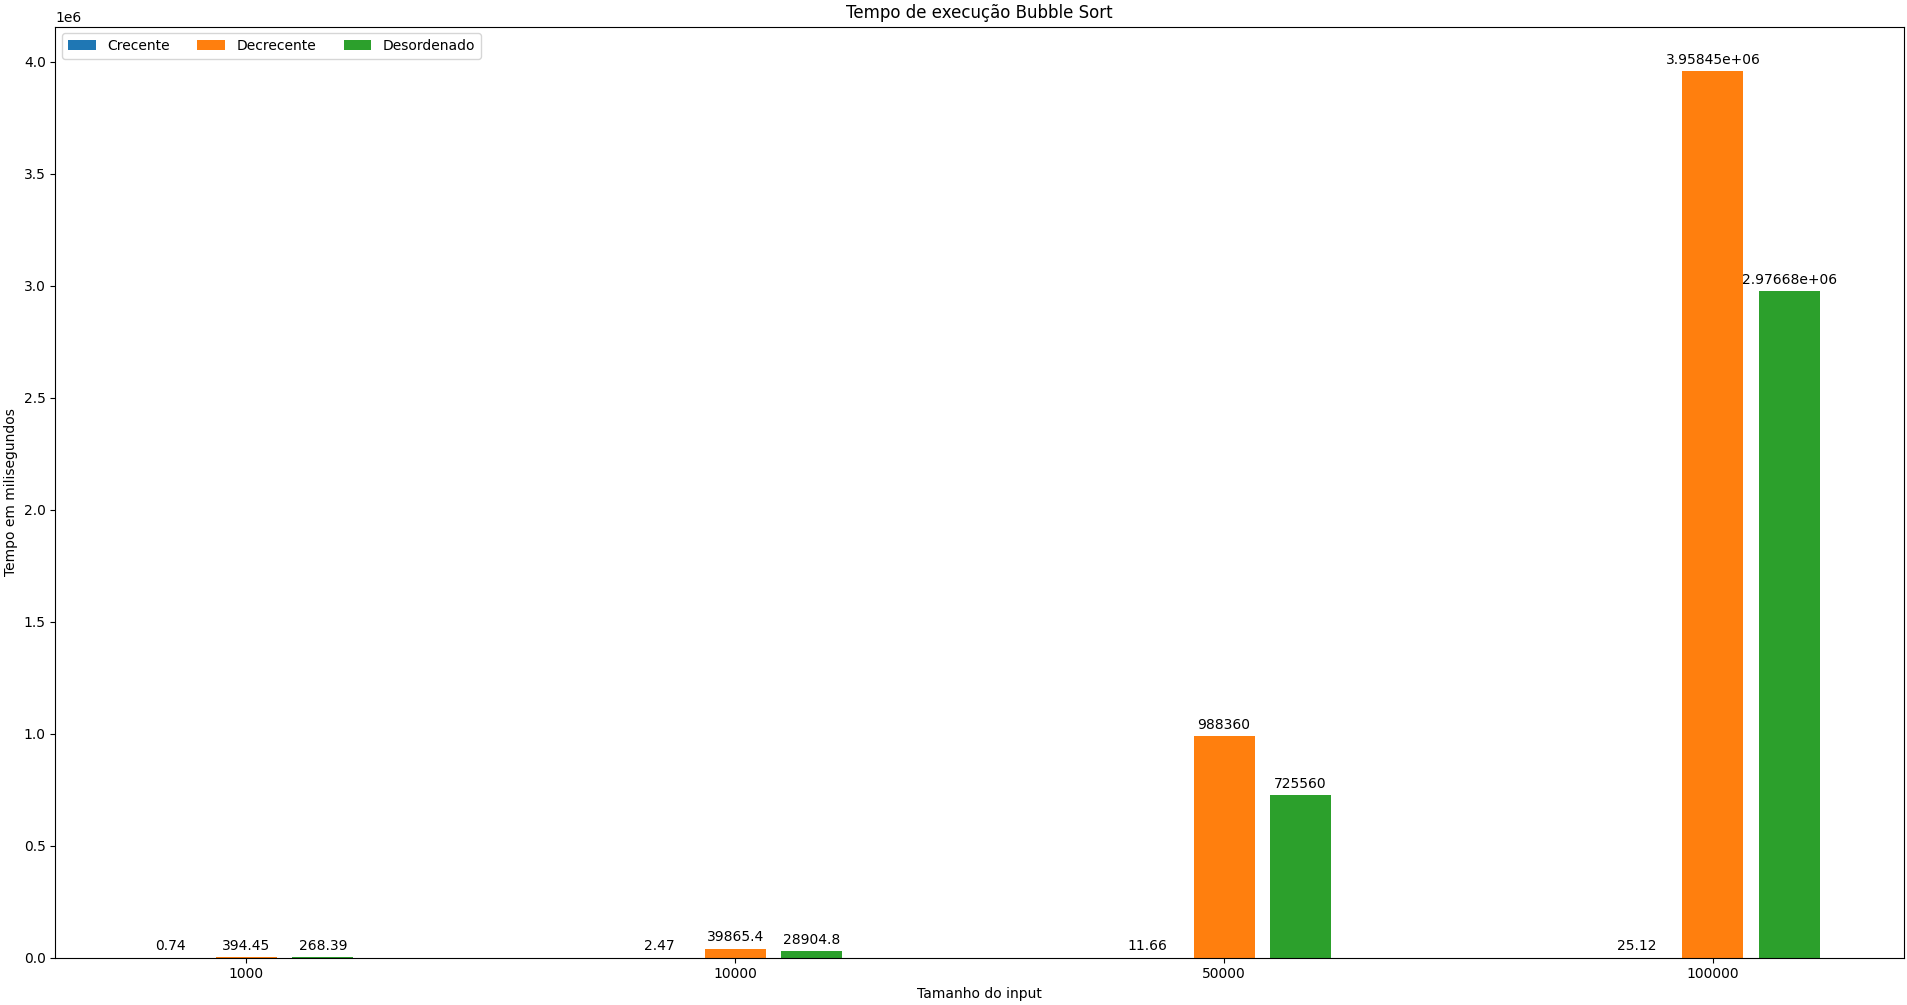
\includegraphics[width=\textwidth]{Graficos/Tempos/BubbleSort.png}
    \caption{Tempo Bubble Sort}
    \label{fig:tempBubbleSort}
\end{figure}

\begin{figure}[H]
    \centering
    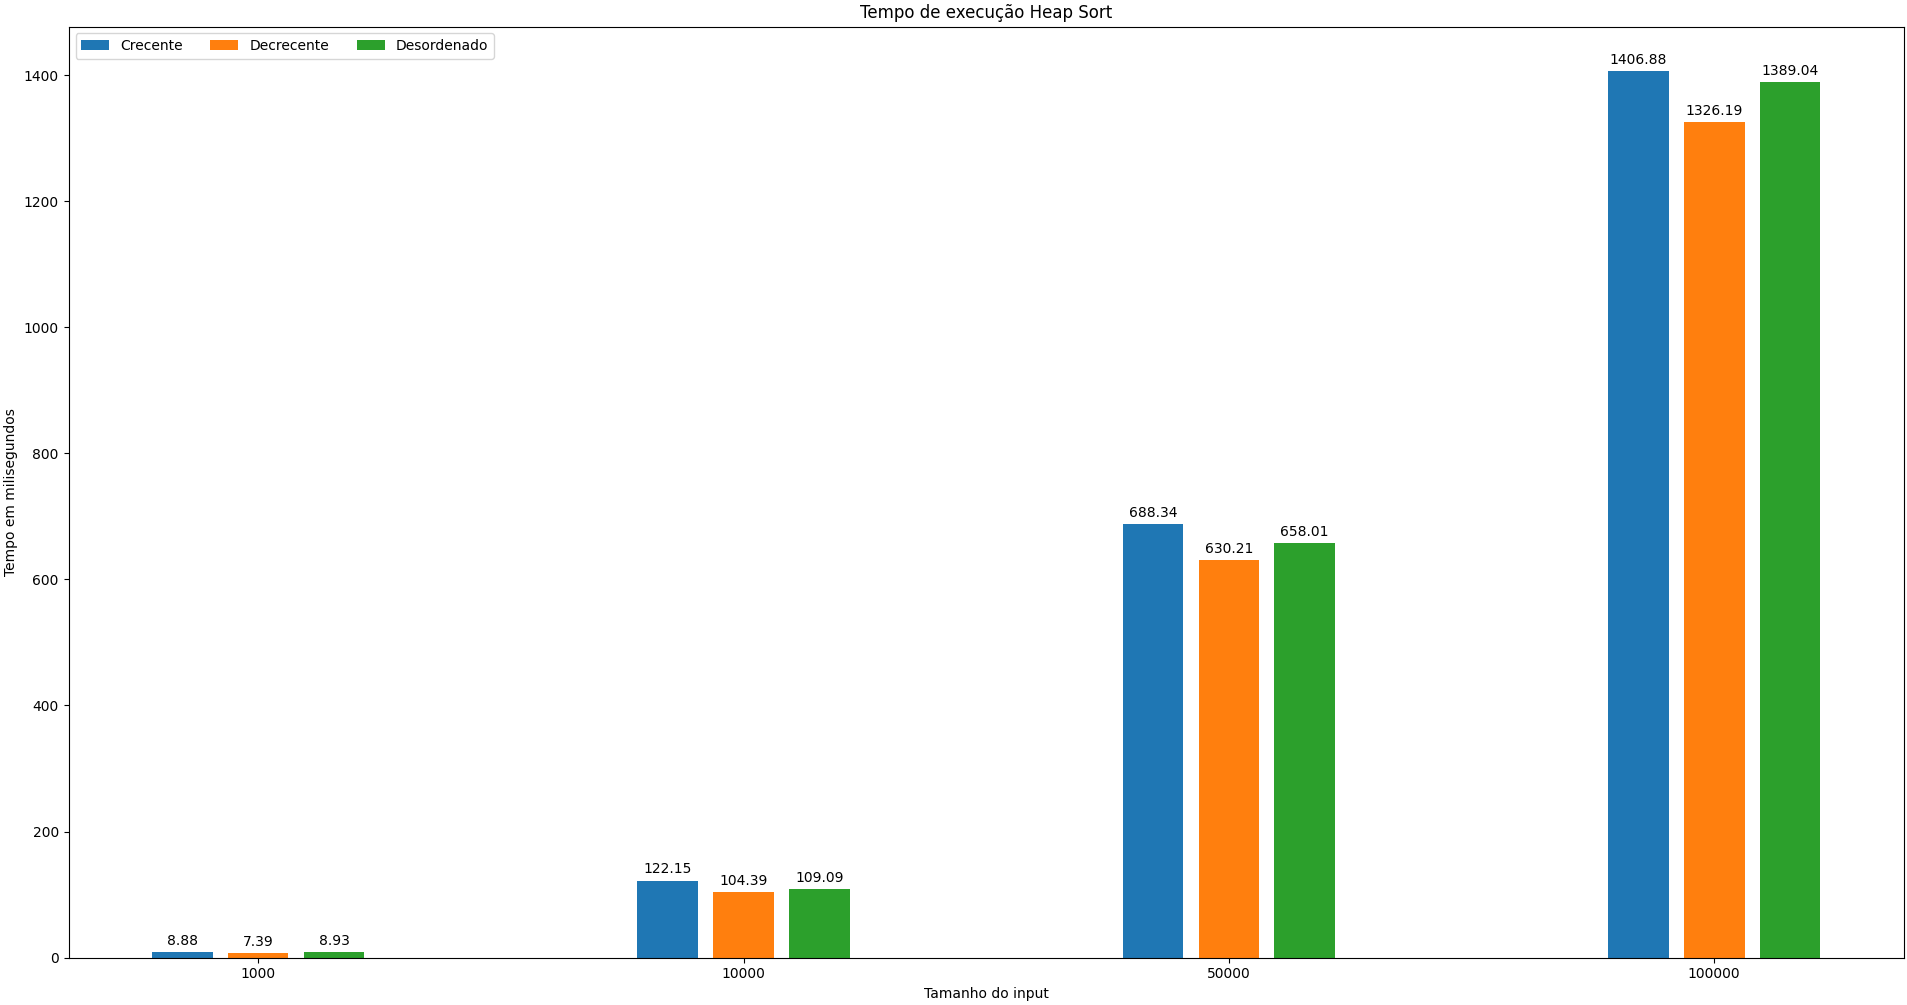
\includegraphics[width=\textwidth]{Graficos/Tempos/HeapSort.png}
    \caption{Tempo HeapSort}
    \label{fig:tempHeapSort}
\end{figure}

\begin{figure}[H]
    \centering
    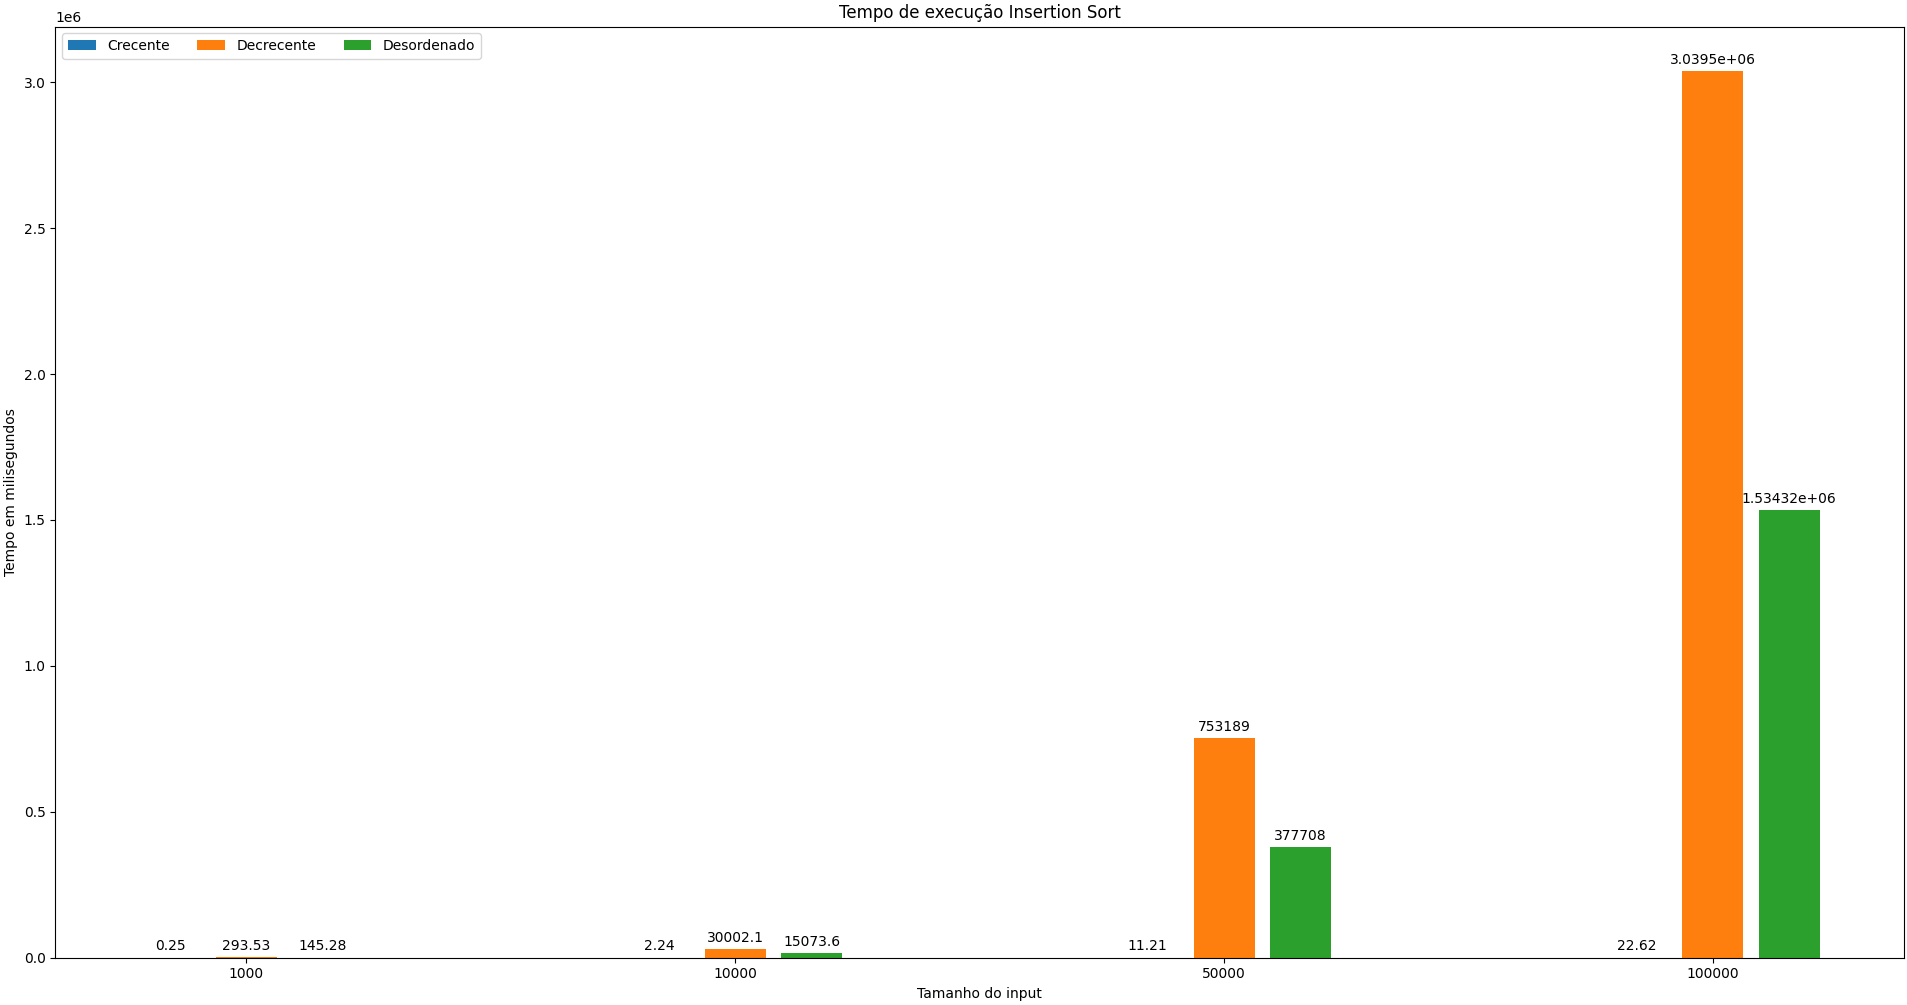
\includegraphics[width=\textwidth]{Graficos/Tempos/InsertionSort.png}
    \caption{Tempo Insertion Sort}
    \label{fig:tempInsertionSort}
\end{figure}

\begin{figure}[H]
    \centering
    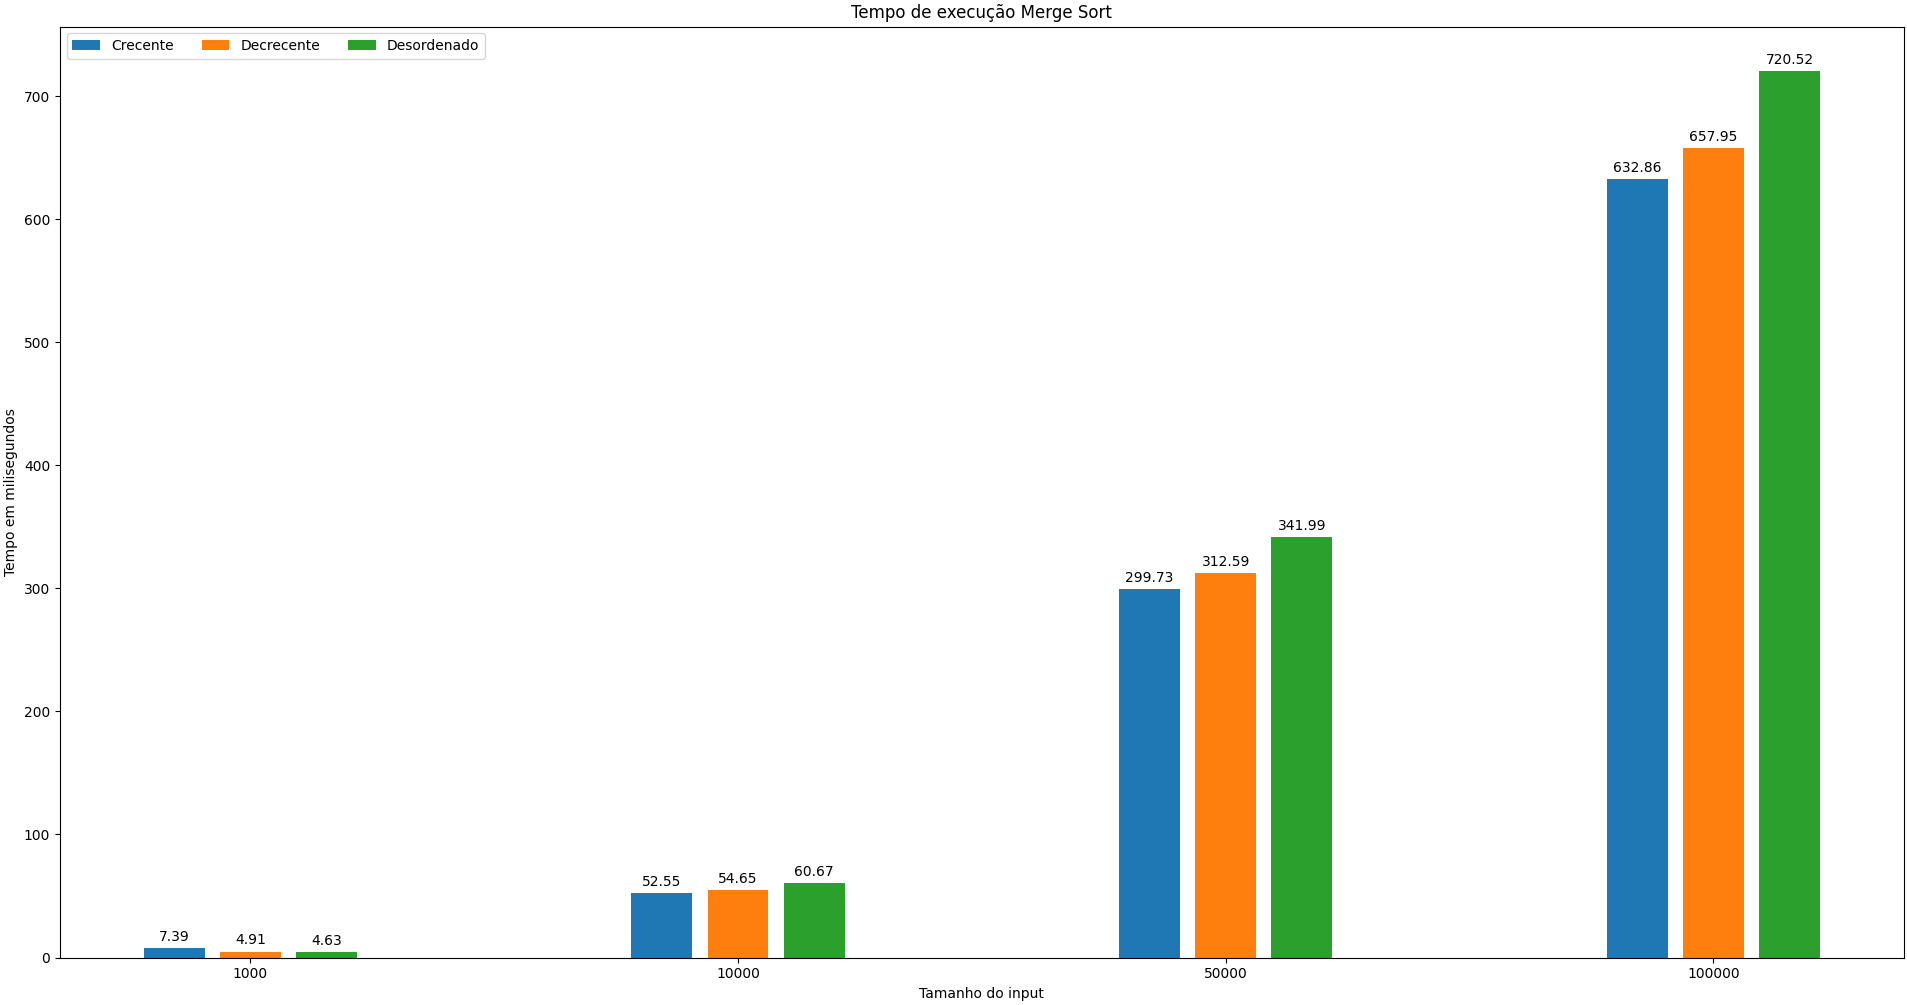
\includegraphics[width=\textwidth]{Graficos/Tempos/MergeSort.png}
    \caption{Tempo Merge Sort}
    \label{fig:tempMergeSort}
\end{figure}

\begin{figure}[H]
    \centering
    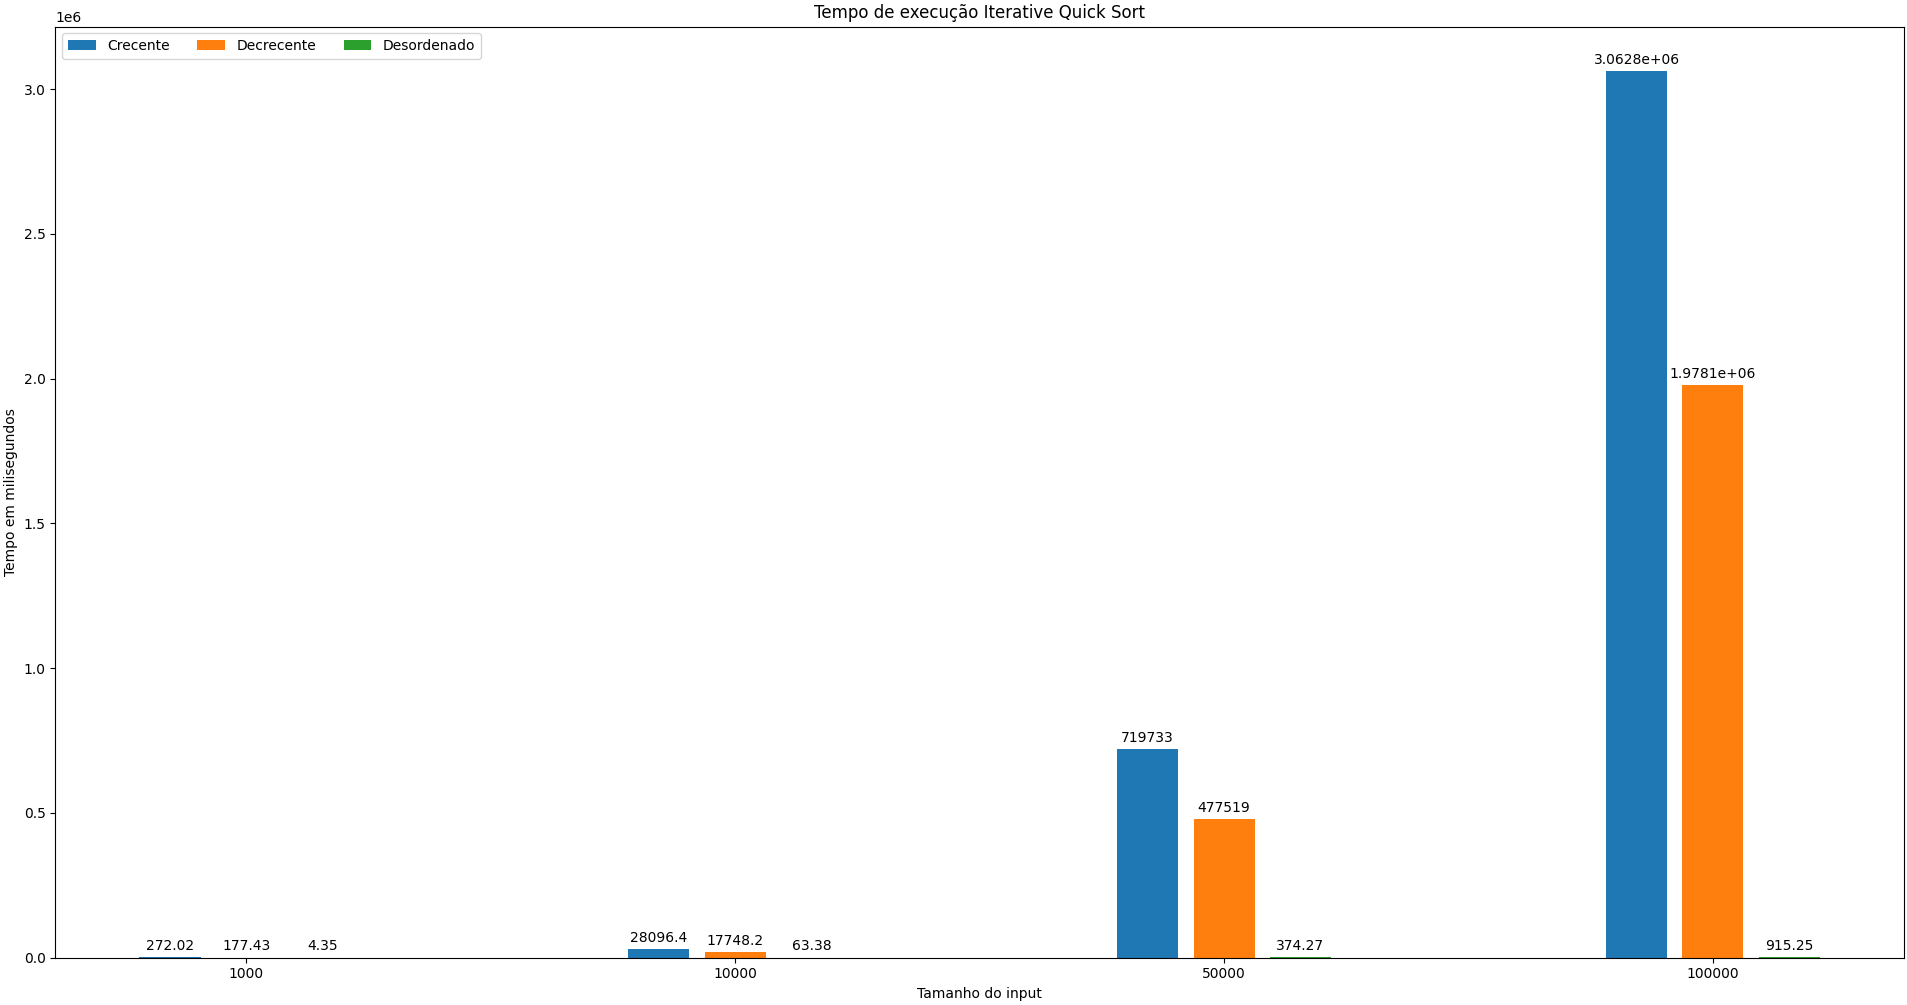
\includegraphics[width=\textwidth]{Graficos/Tempos/QuickSort.png}
    \caption{Tempo Quick Sort}
    \label{fig:tempQuickSort}
\end{figure}

\begin{figure}[H]
    \centering
    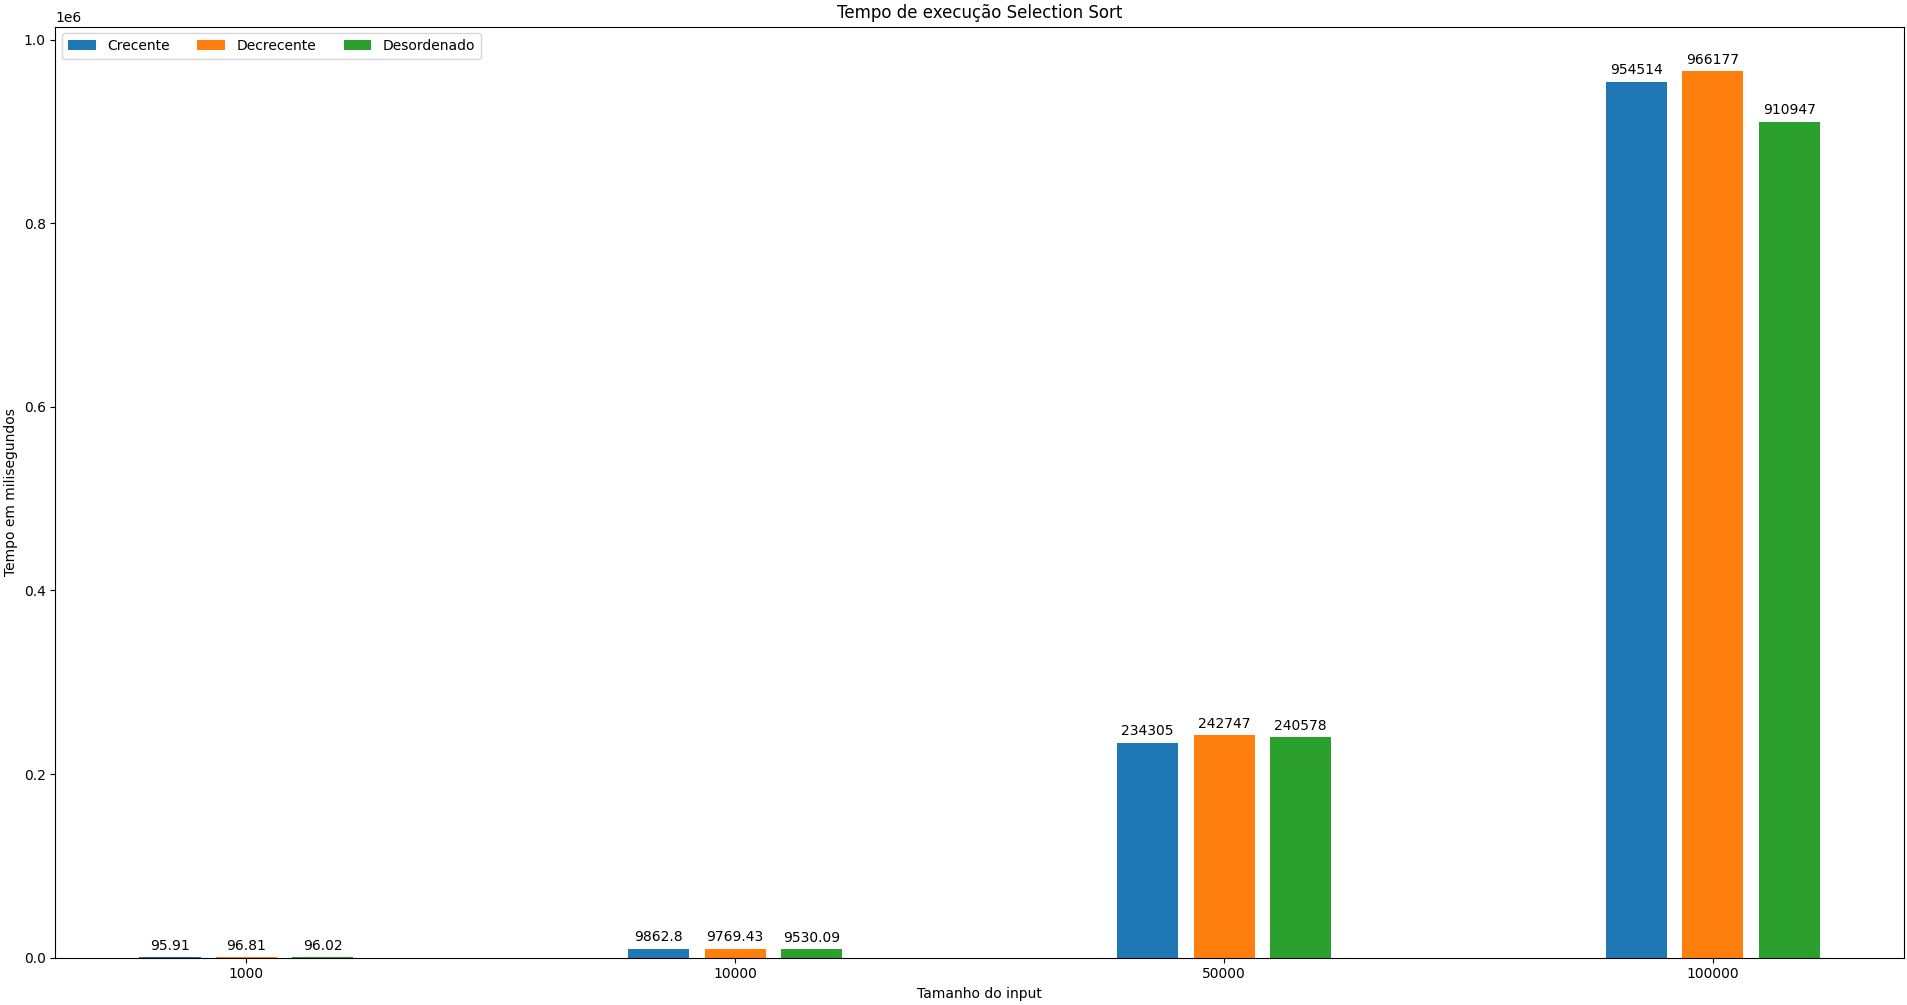
\includegraphics[width=\textwidth]{Graficos/Tempos/SelectionSort.png}
    \caption{Tempo Selection Sort}
    \label{fig:tempSelectionSort}
\end{figure}

\subsubsection{Gráficos das comparações dos algoritmos}
\begin{figure}[H]
    \centering
    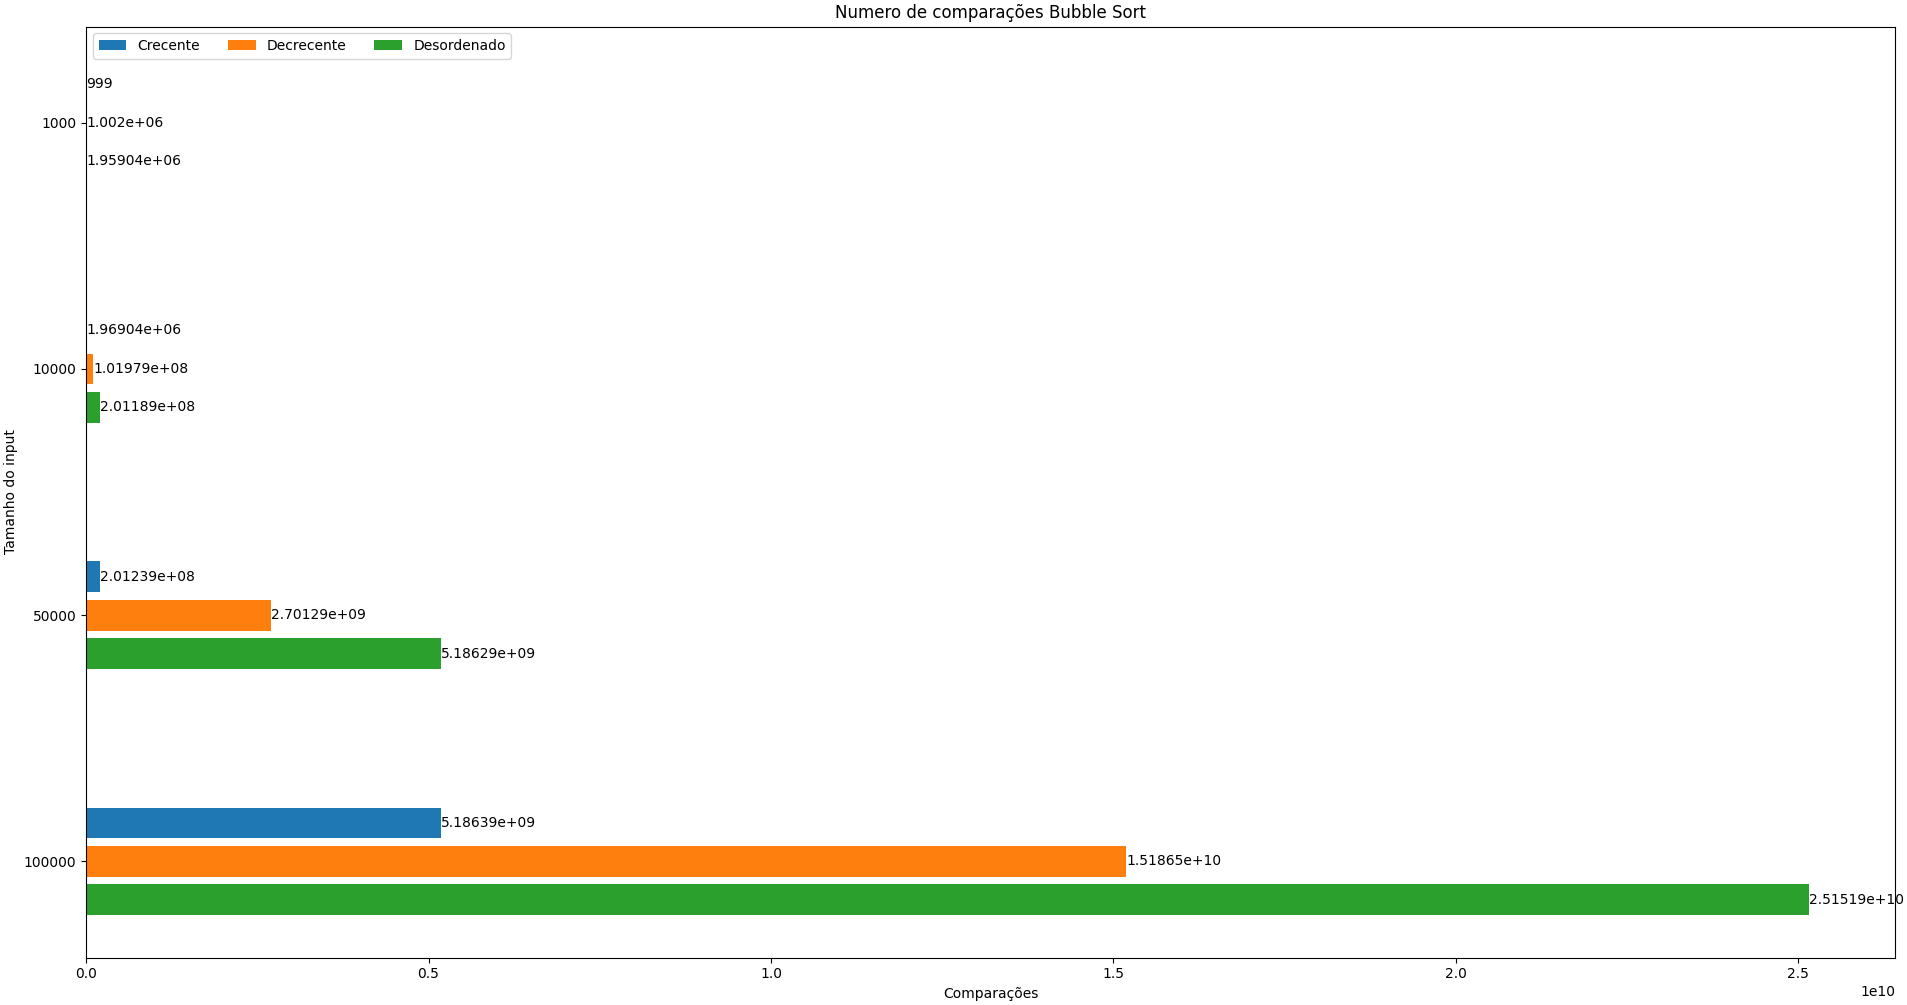
\includegraphics[width=\textwidth]{Graficos/Comparações/Bubble Sort.png}
    \caption{Comparações Bubble Sort}
    \label{fig:compBubbleSort}
\end{figure}

\begin{figure}[H]
    \centering
    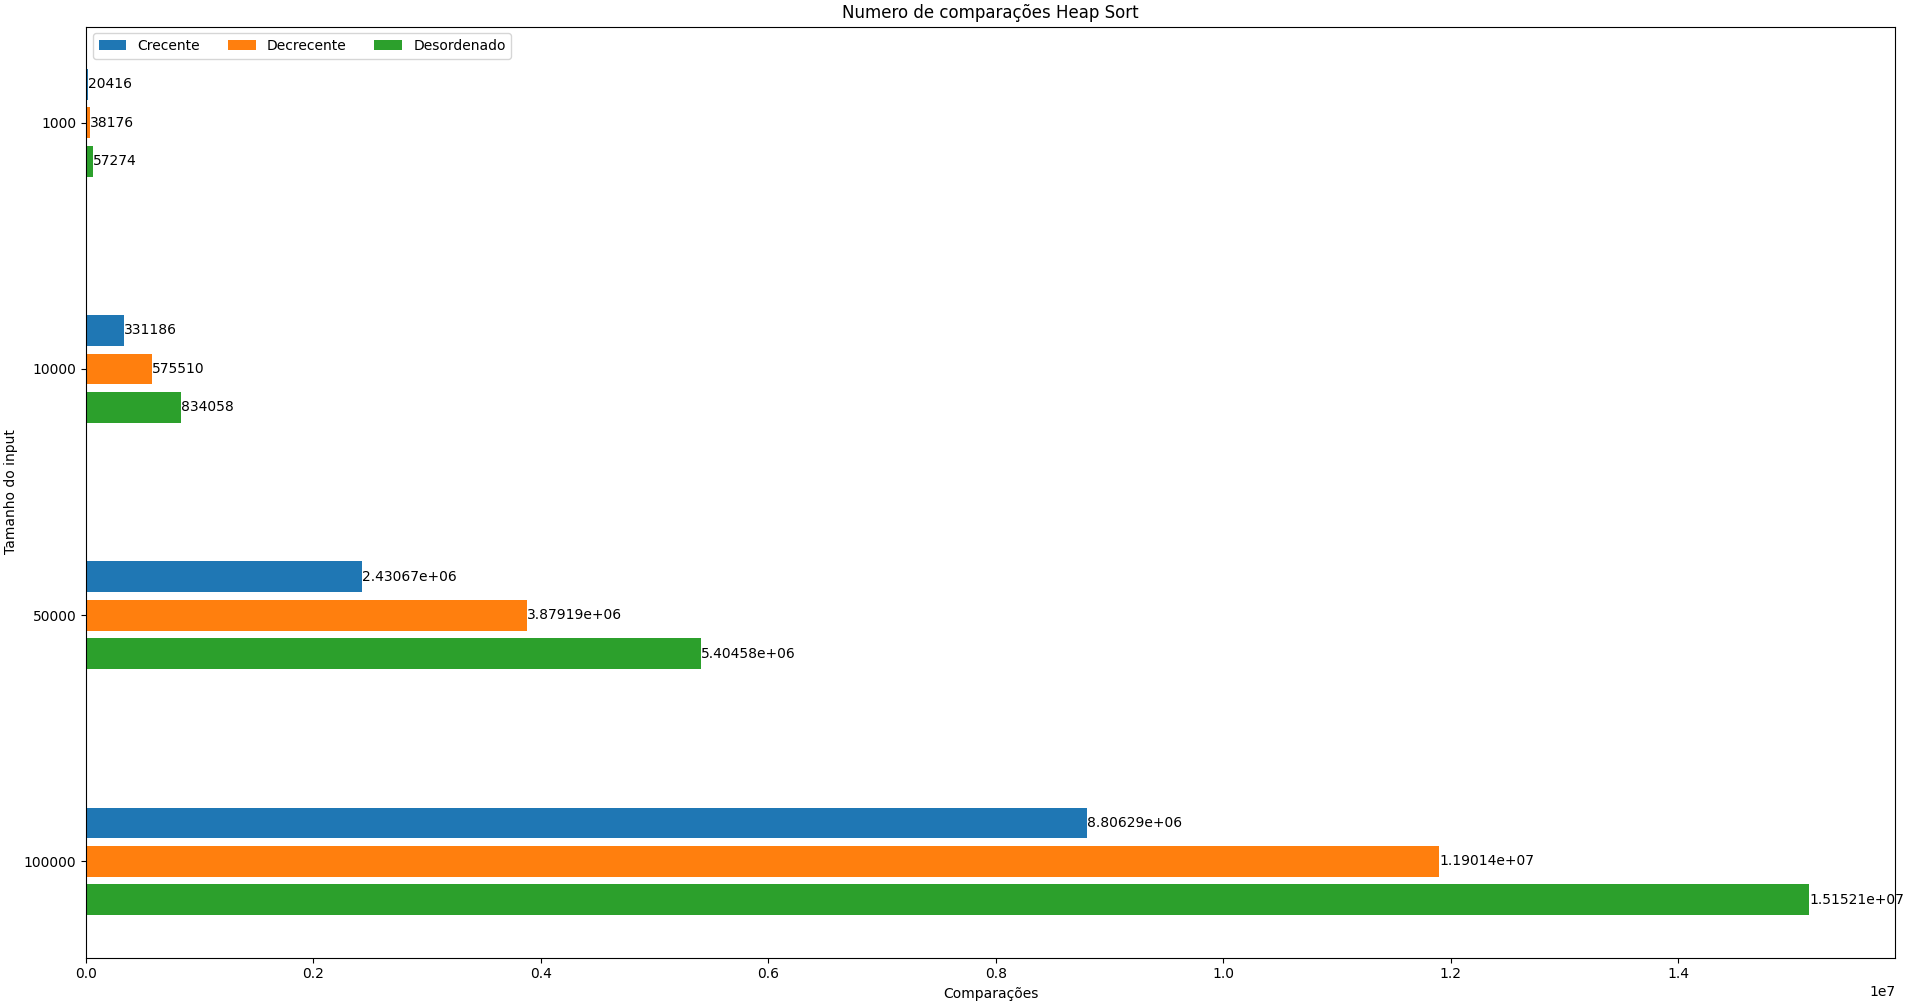
\includegraphics[width=\textwidth]{Graficos/Comparações/Heap Sort.png}
    \caption{Comparações HeapSort}
    \label{fig:compHeapSort}
\end{figure}

\begin{figure}[H]
    \centering
    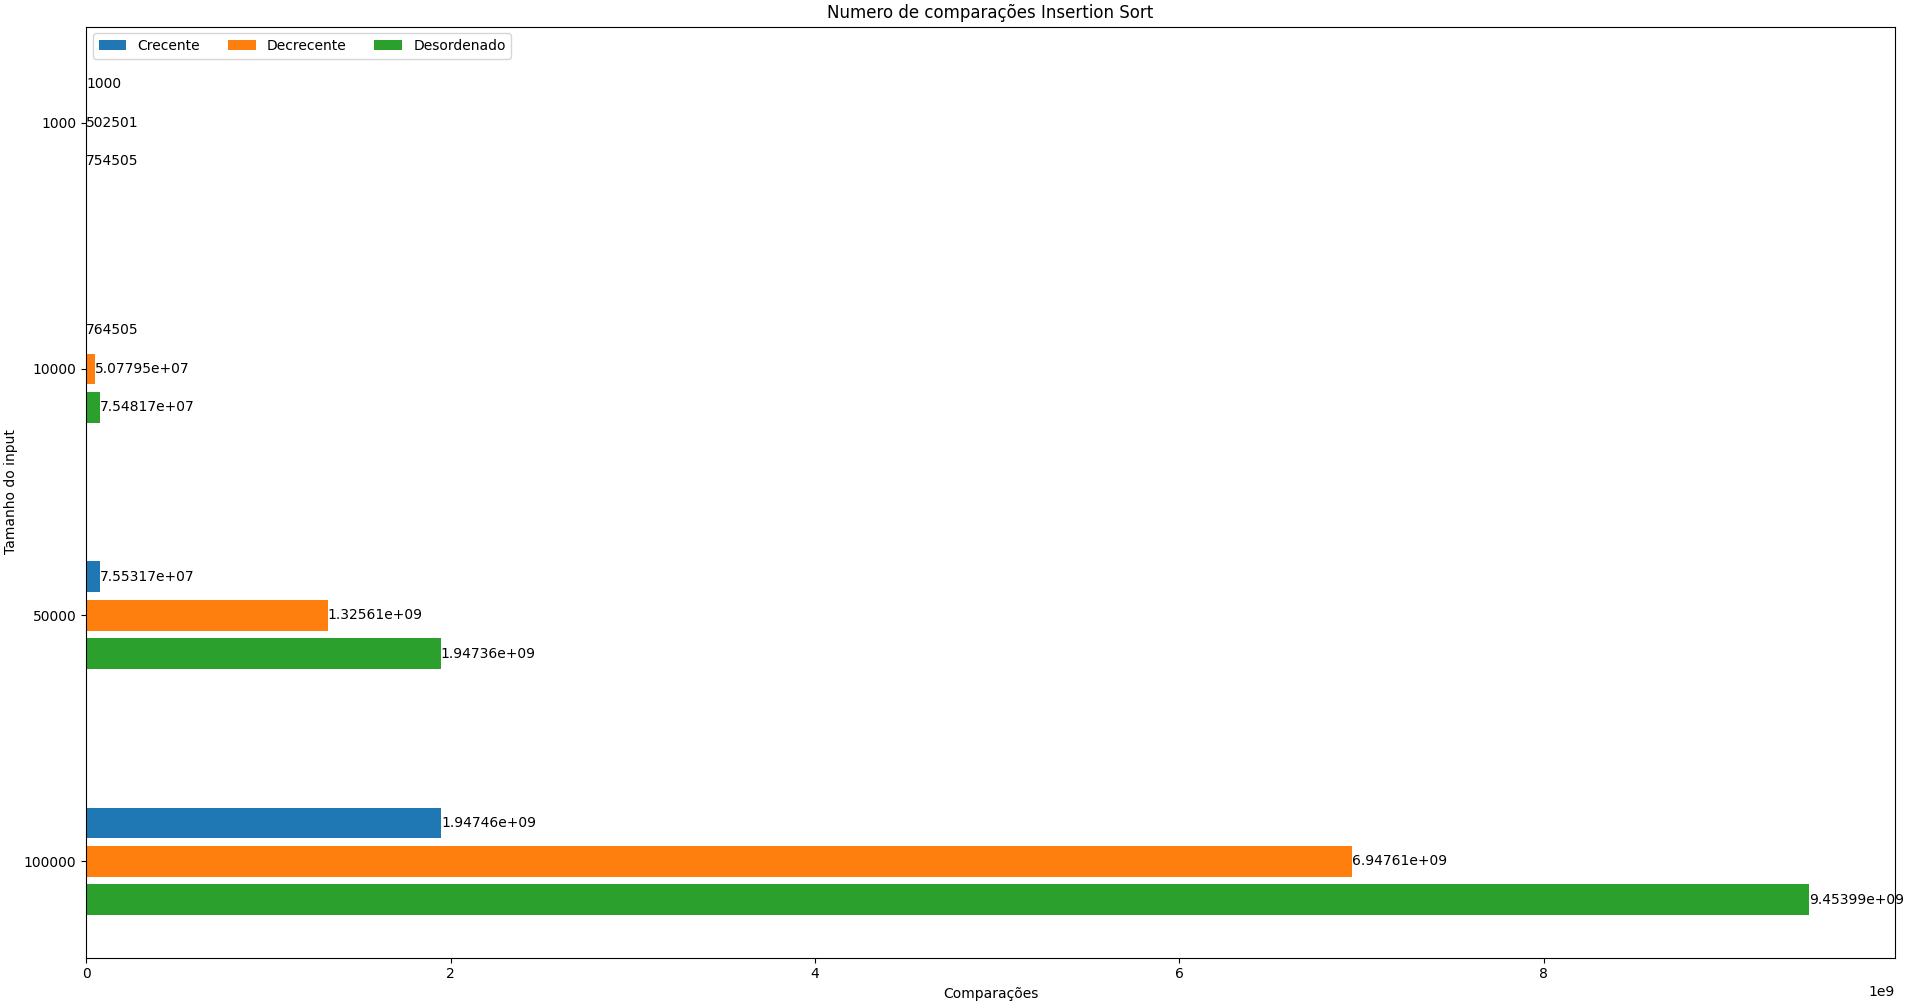
\includegraphics[width=\textwidth]{Graficos/Comparações/Insertion Sort.png}
    \caption{Comparações Insertion Sort}
    \label{fig:compInsertionSort}
\end{figure}

\begin{figure}[H]
    \centering
    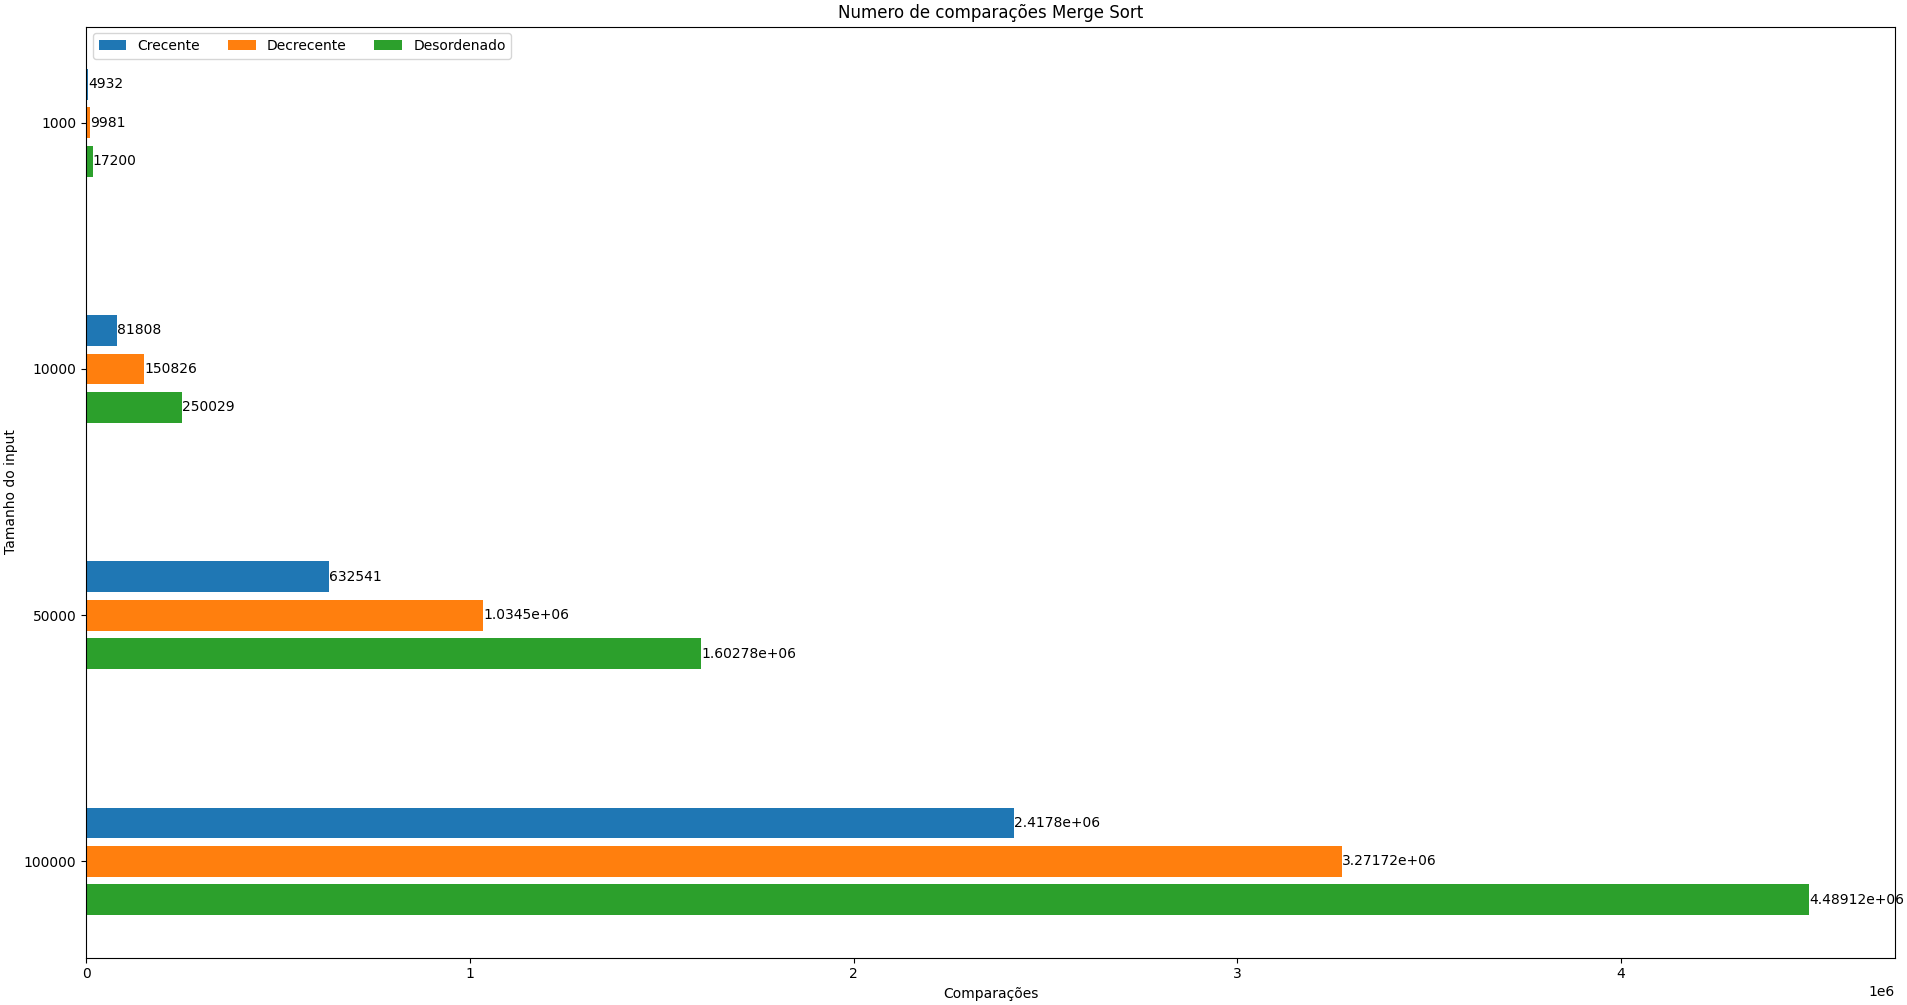
\includegraphics[width=\textwidth]{Graficos/Comparações/Merge Sort.png}
    \caption{Comparações Merge Sort}
    \label{fig:compMergeSort}
\end{figure}

\begin{figure}[H]
    \centering
    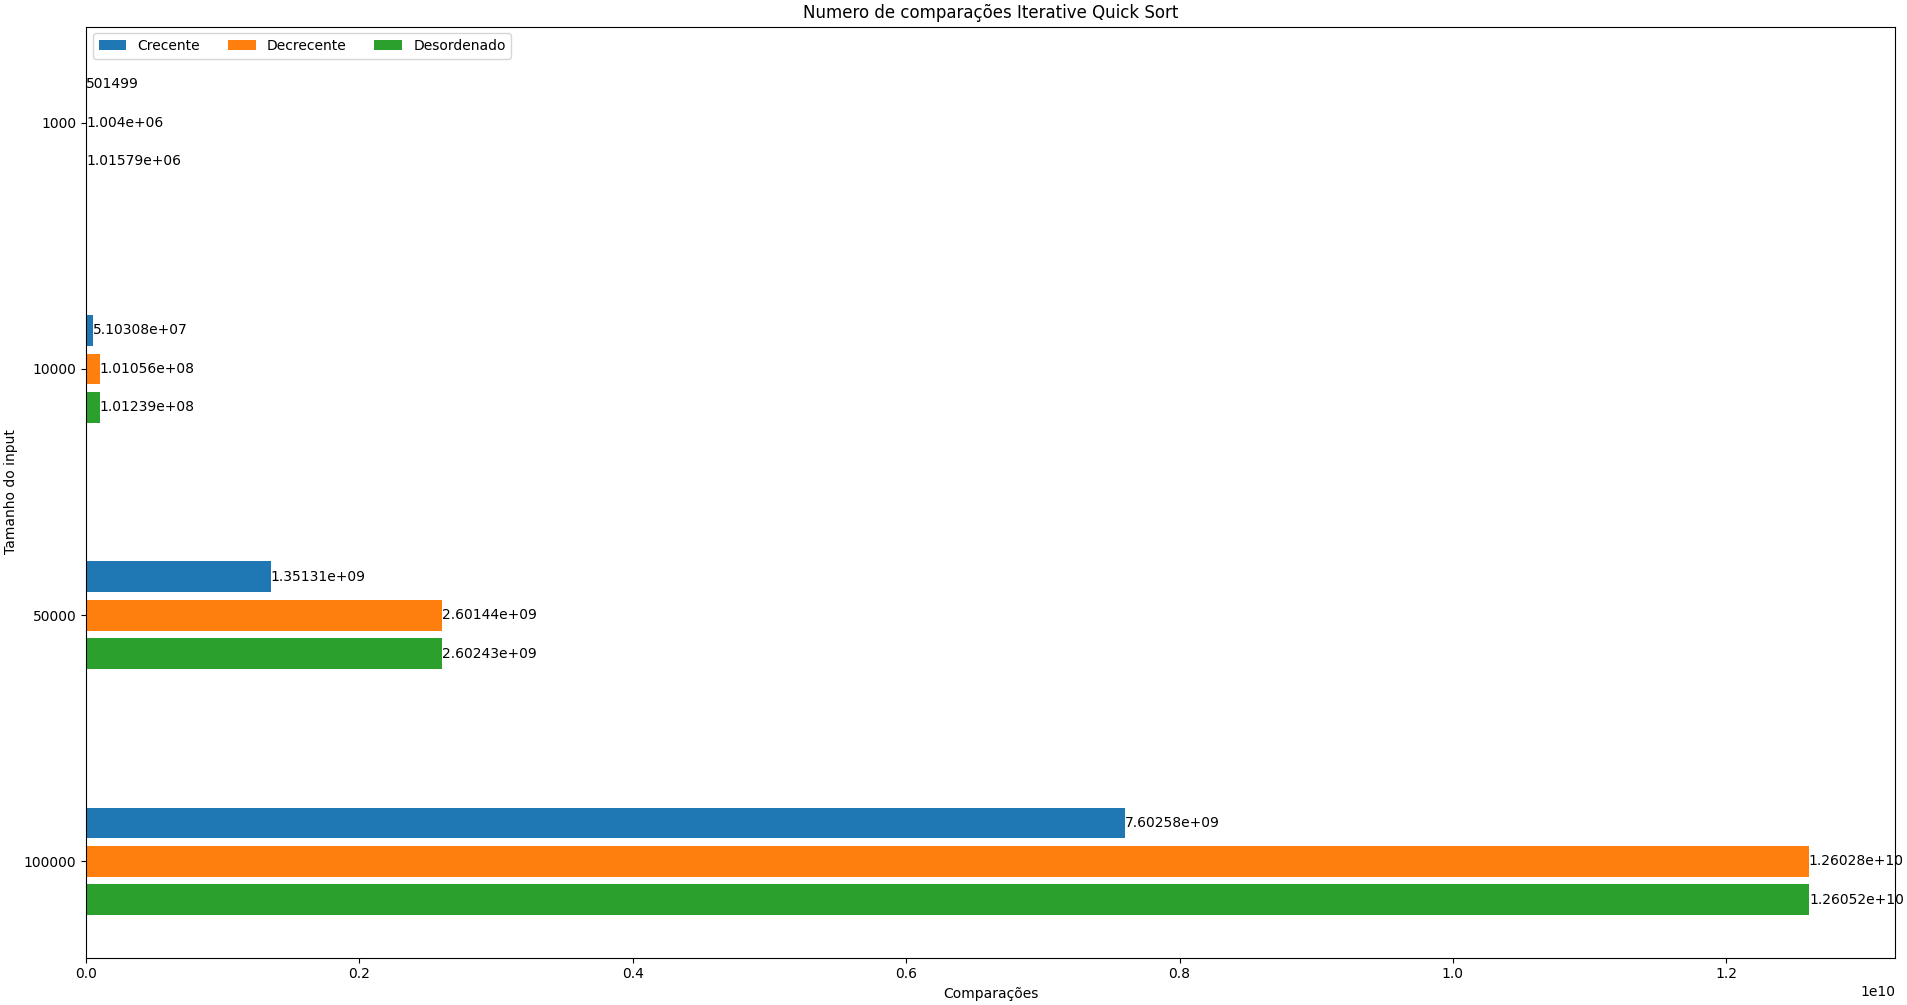
\includegraphics[width=\textwidth]{Graficos/Comparações/Iterative Quick Sort.png}
    \caption{Comparações Quick Sort}
    \label{fig:compQuickSort}
\end{figure}

\begin{figure}[H]
    \centering
    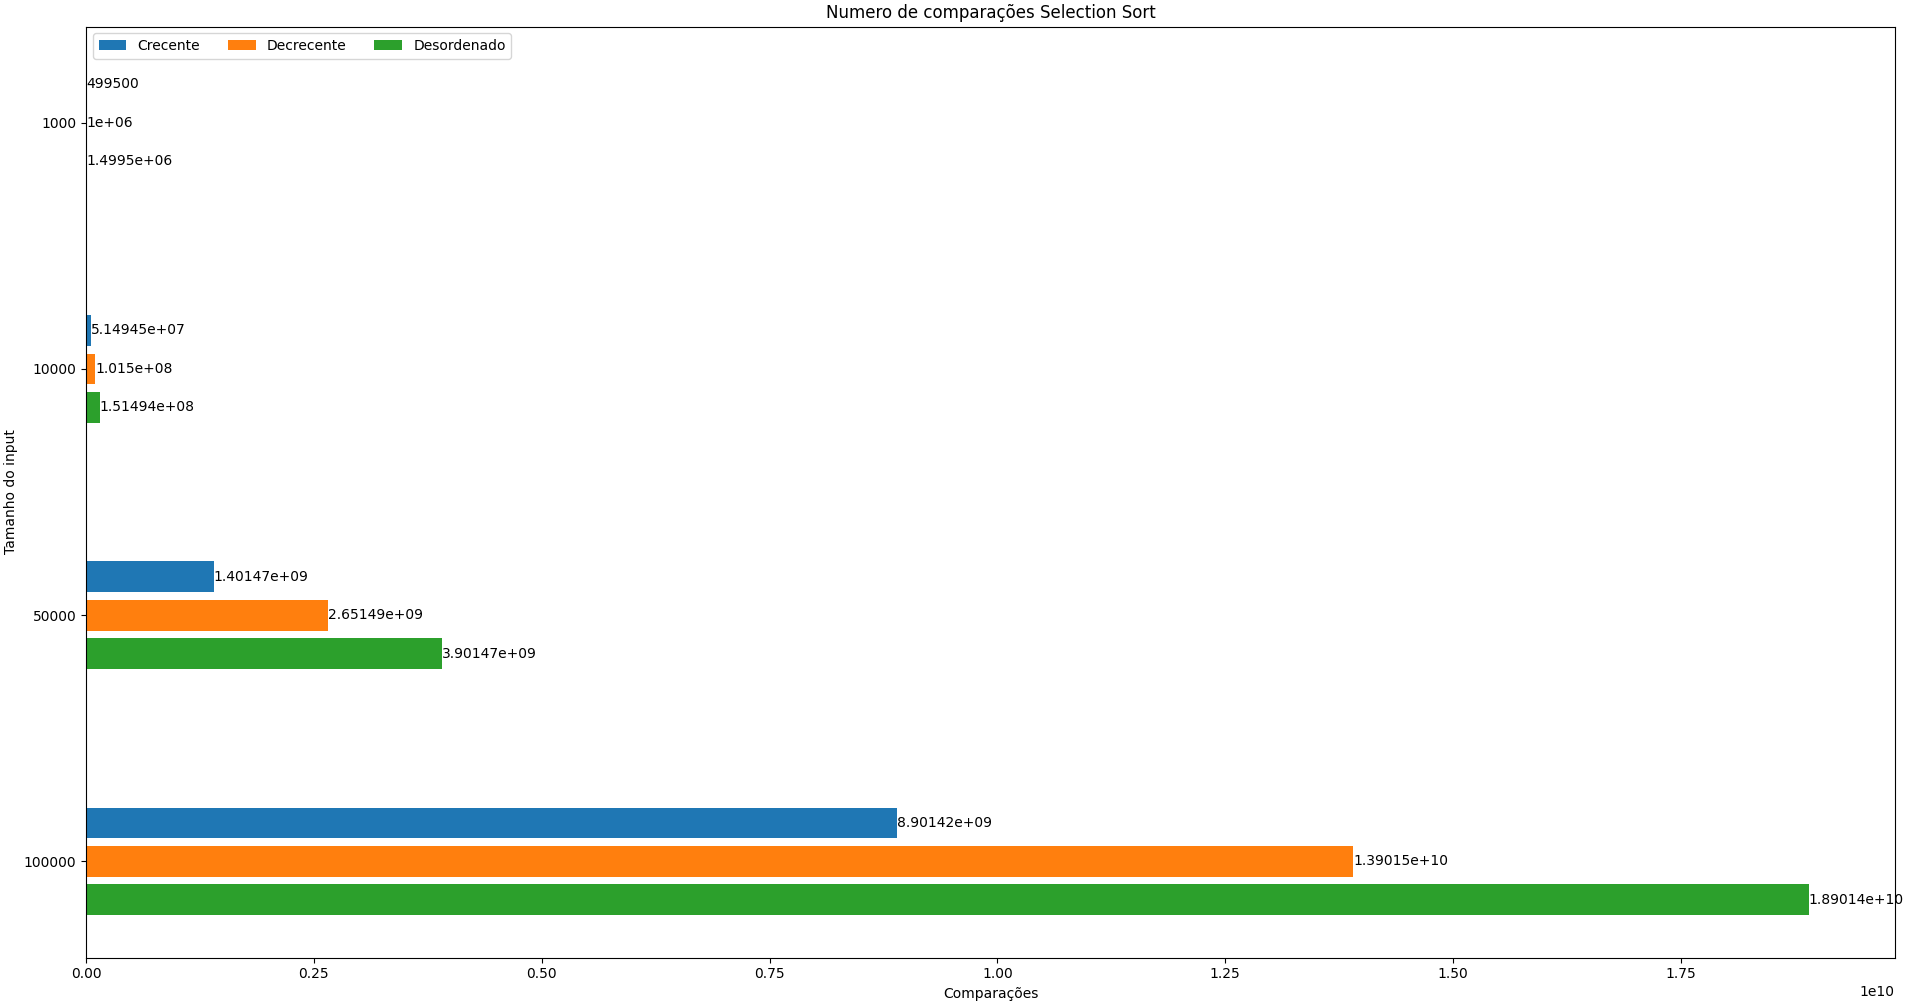
\includegraphics[width=\textwidth]{Graficos/Comparações/Selection Sort.png}
    \caption{Comparações Selection Sort}
    \label{fig:compSelectionSort}
\end{figure}

\subsubsection{Gráficos das trocas dos algoritmos}
\begin{figure}[H]
    \centering
    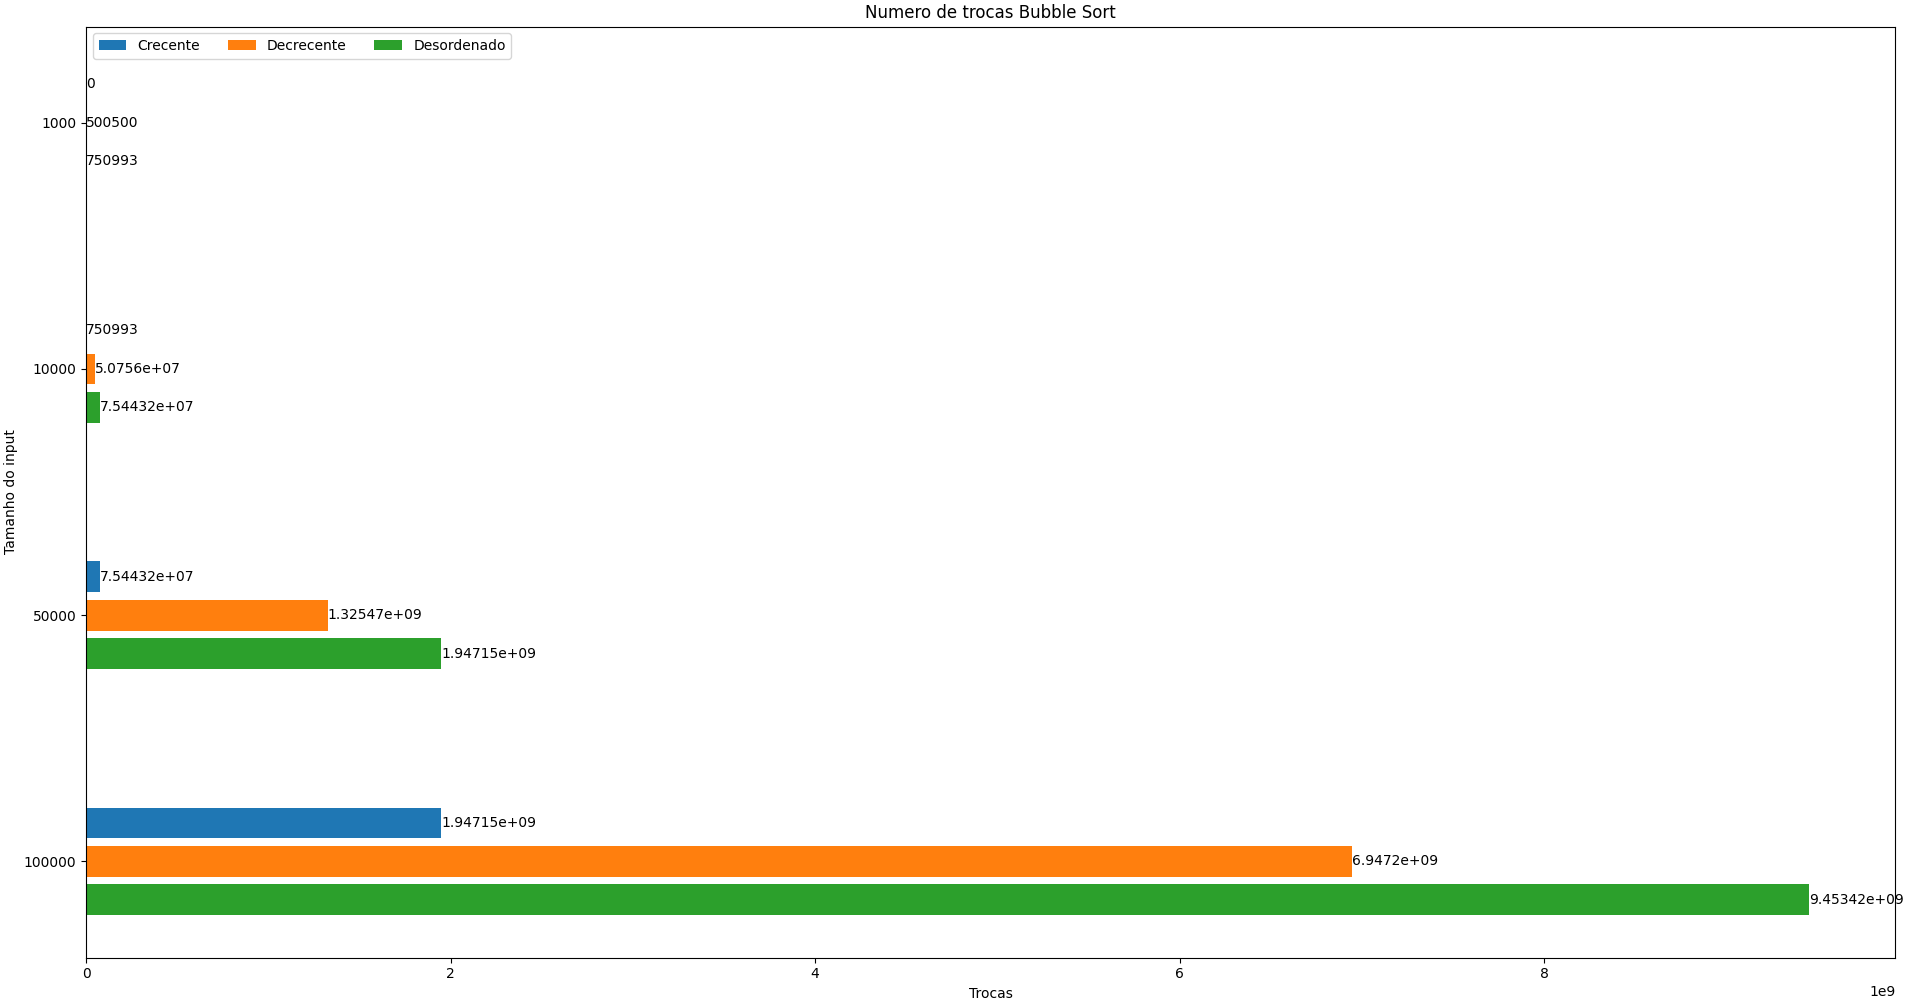
\includegraphics[width=\textwidth]{Graficos/Trocas/Bubble Sort.png}
    \caption{Trocas Bubble Sort}
    \label{fig:trocasBubbleSort}
\end{figure}

\begin{figure}[H]
    \centering
    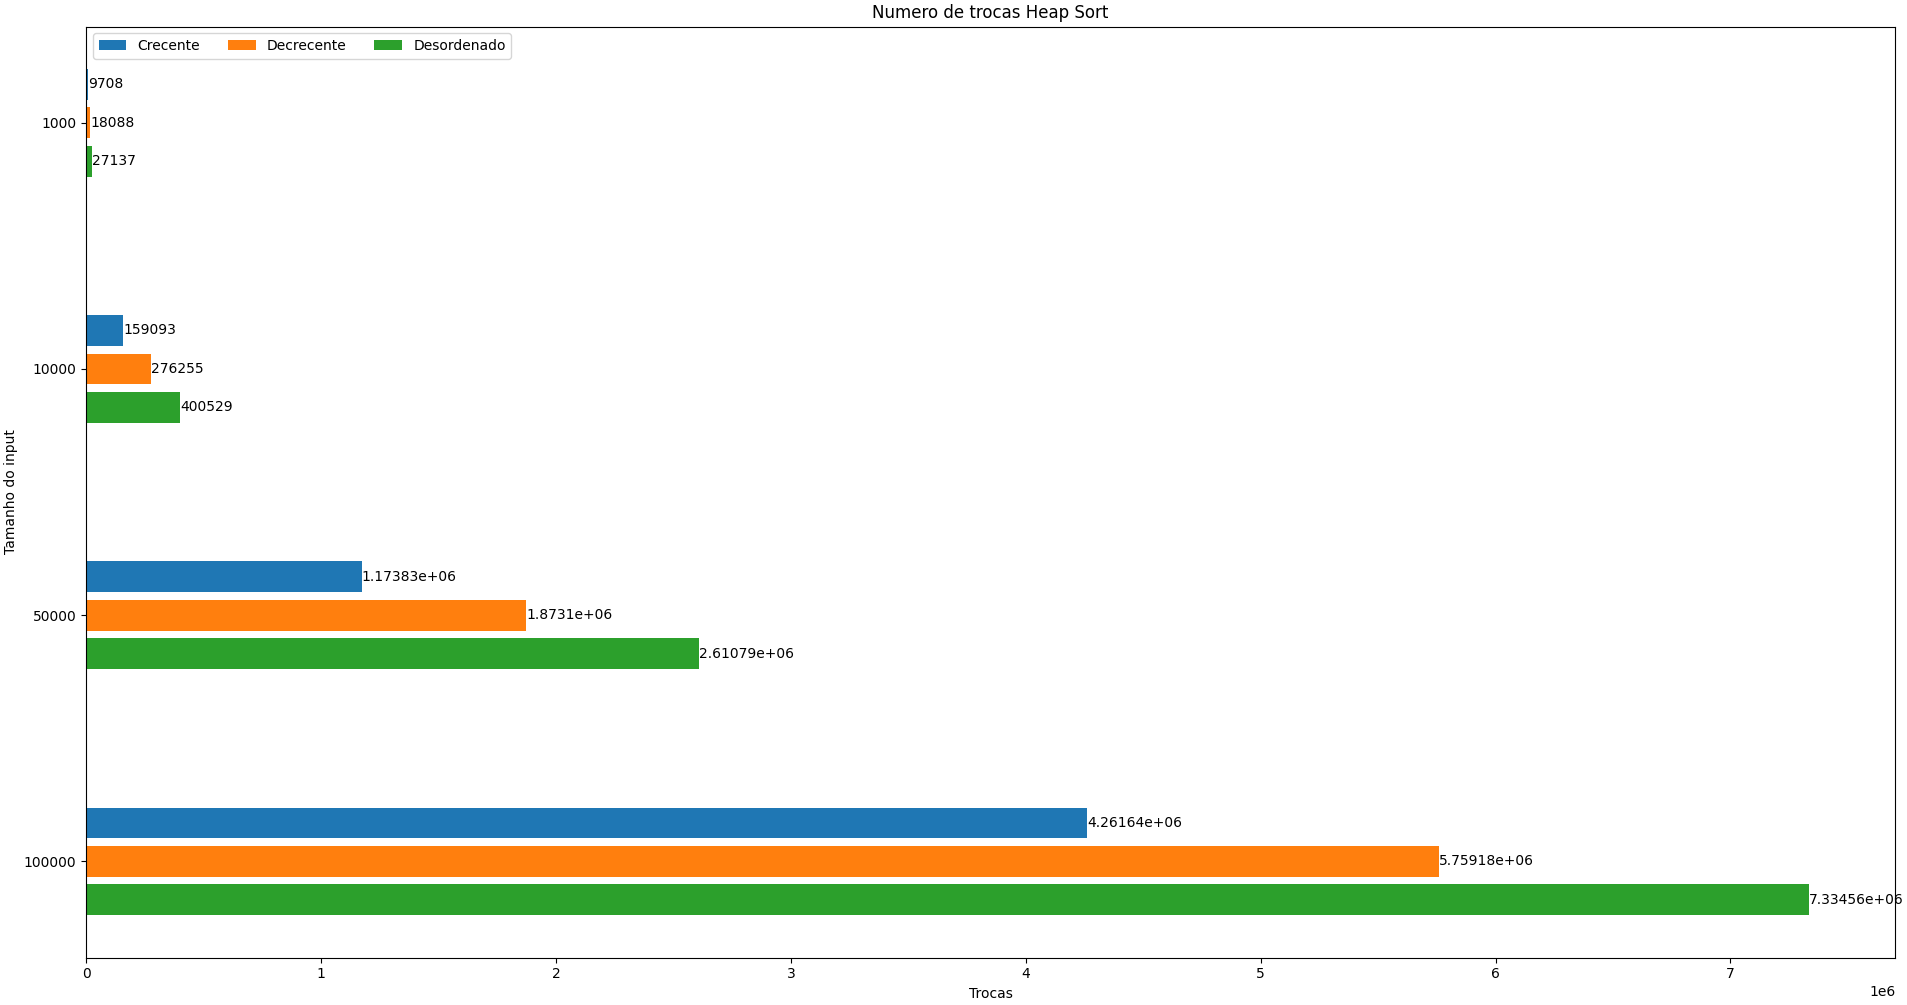
\includegraphics[width=\textwidth]{Graficos/Trocas/Heap Sort.png}
    \caption{Trocas HeapSort}
    \label{fig:trocasHeapSort}
\end{figure}

\begin{figure}[H]
    \centering
    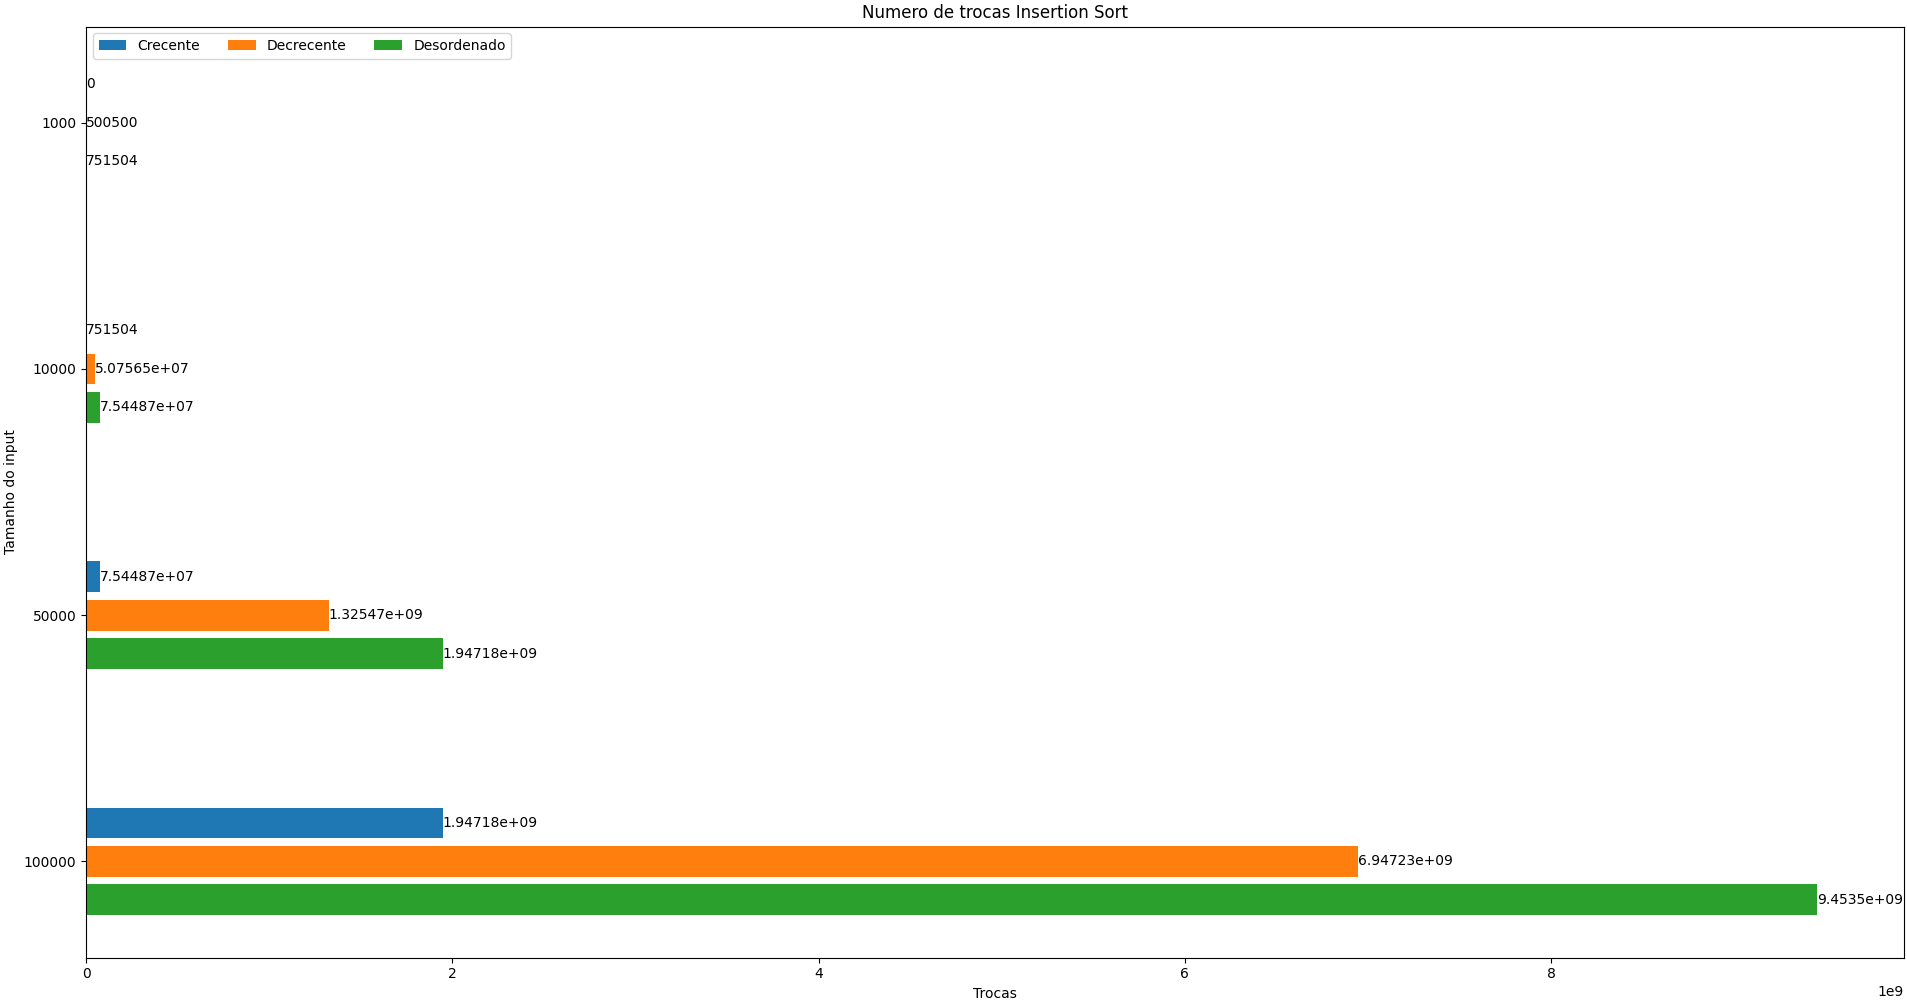
\includegraphics[width=\textwidth]{Graficos/Trocas/Insertion Sort.png}
    \caption{Trocas Insertion Sort}
    \label{fig:trocasInsertionSort}
\end{figure}

\begin{figure}[H]
    \centering
    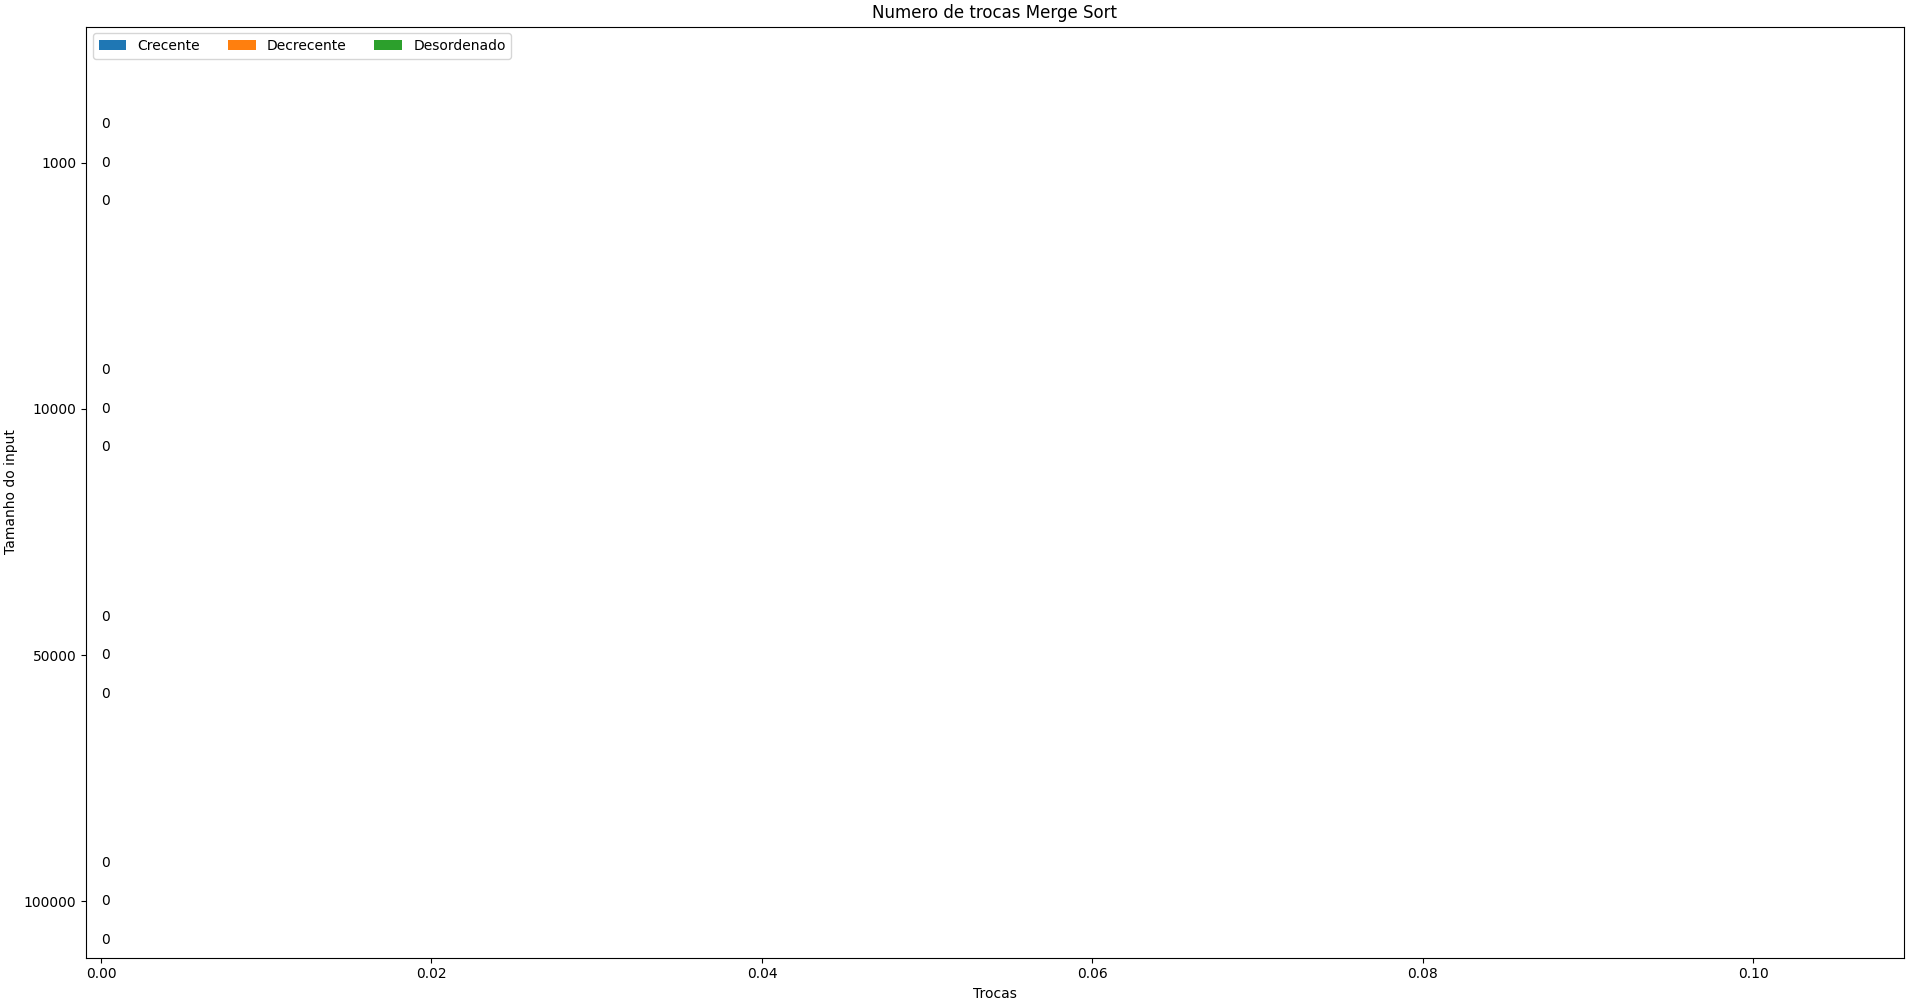
\includegraphics[width=\textwidth]{Graficos/Trocas/Merge Sort.png}
    \caption{Trocas Merge Sort}
    \label{fig:trocasMergeSort}
\end{figure}

\begin{figure}[H]
    \centering
    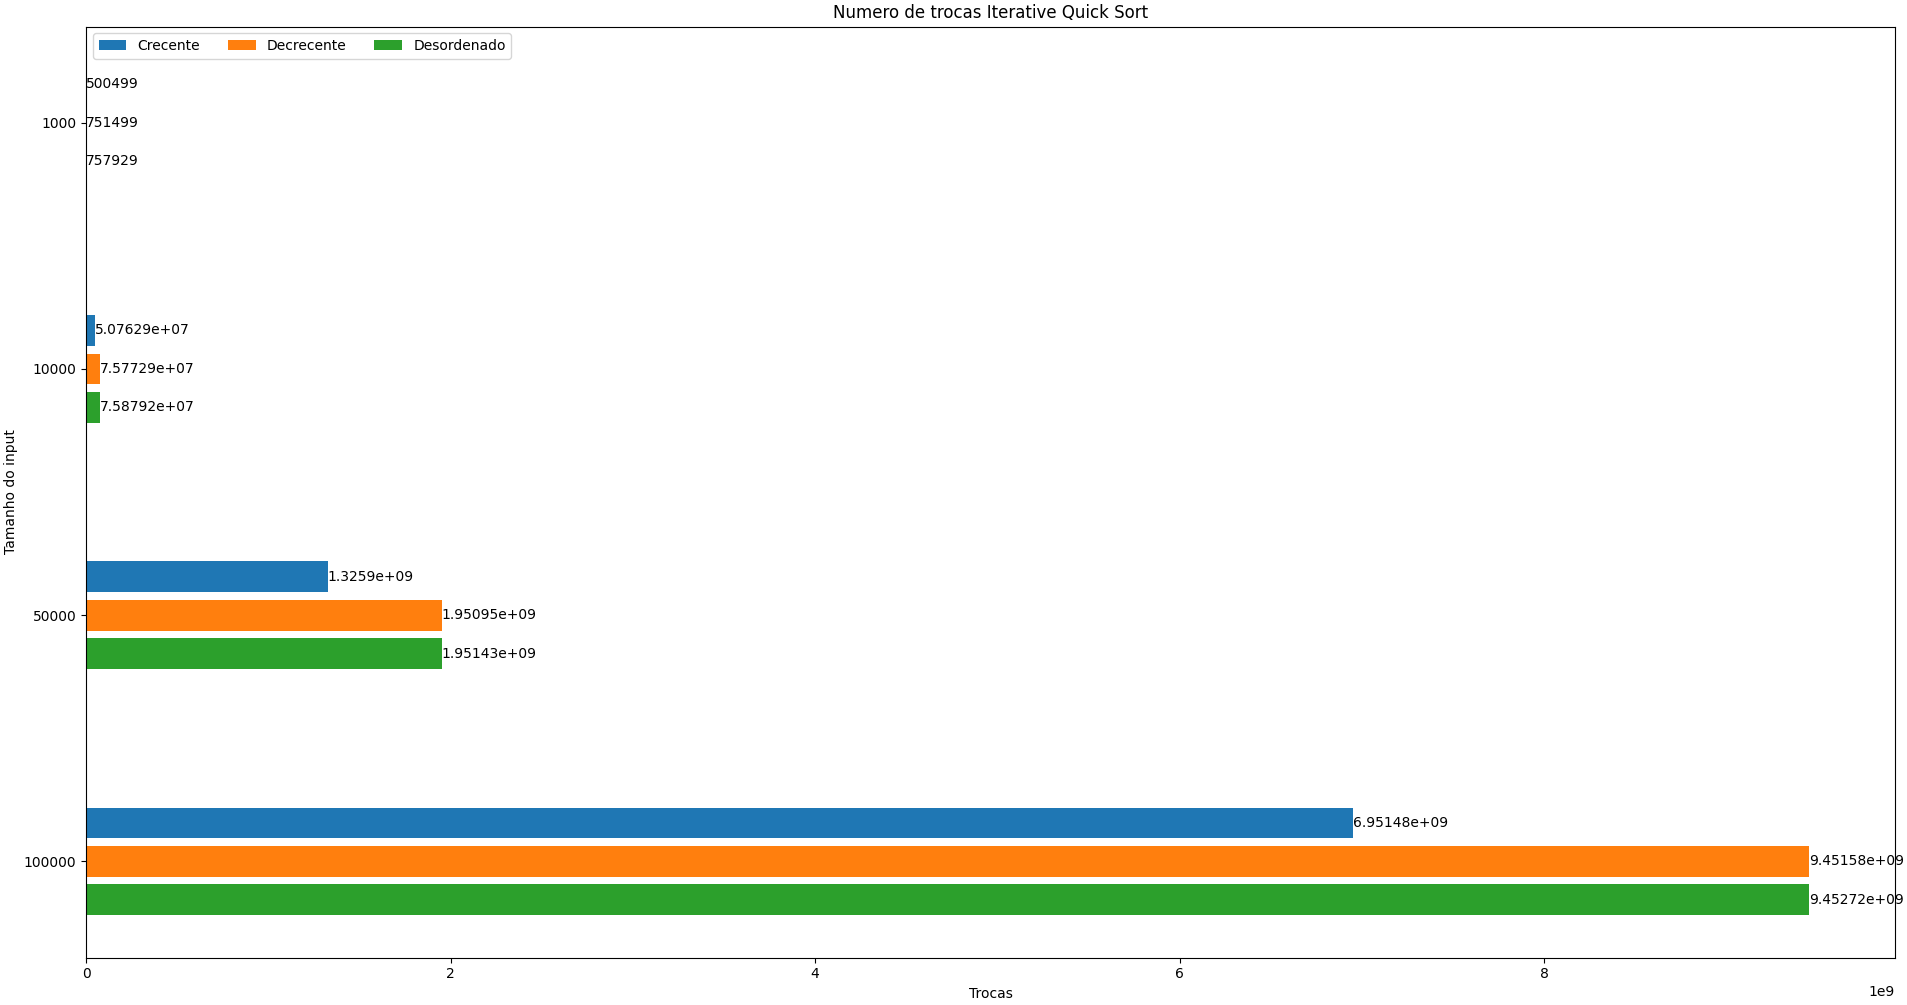
\includegraphics[width=\textwidth]{Graficos/Trocas/Iterative Quick Sort.png}
    \caption{Trocas Quick Sort}
    \label{fig:trocasQuickSort}
\end{figure}

\begin{figure}[H]
    \centering
    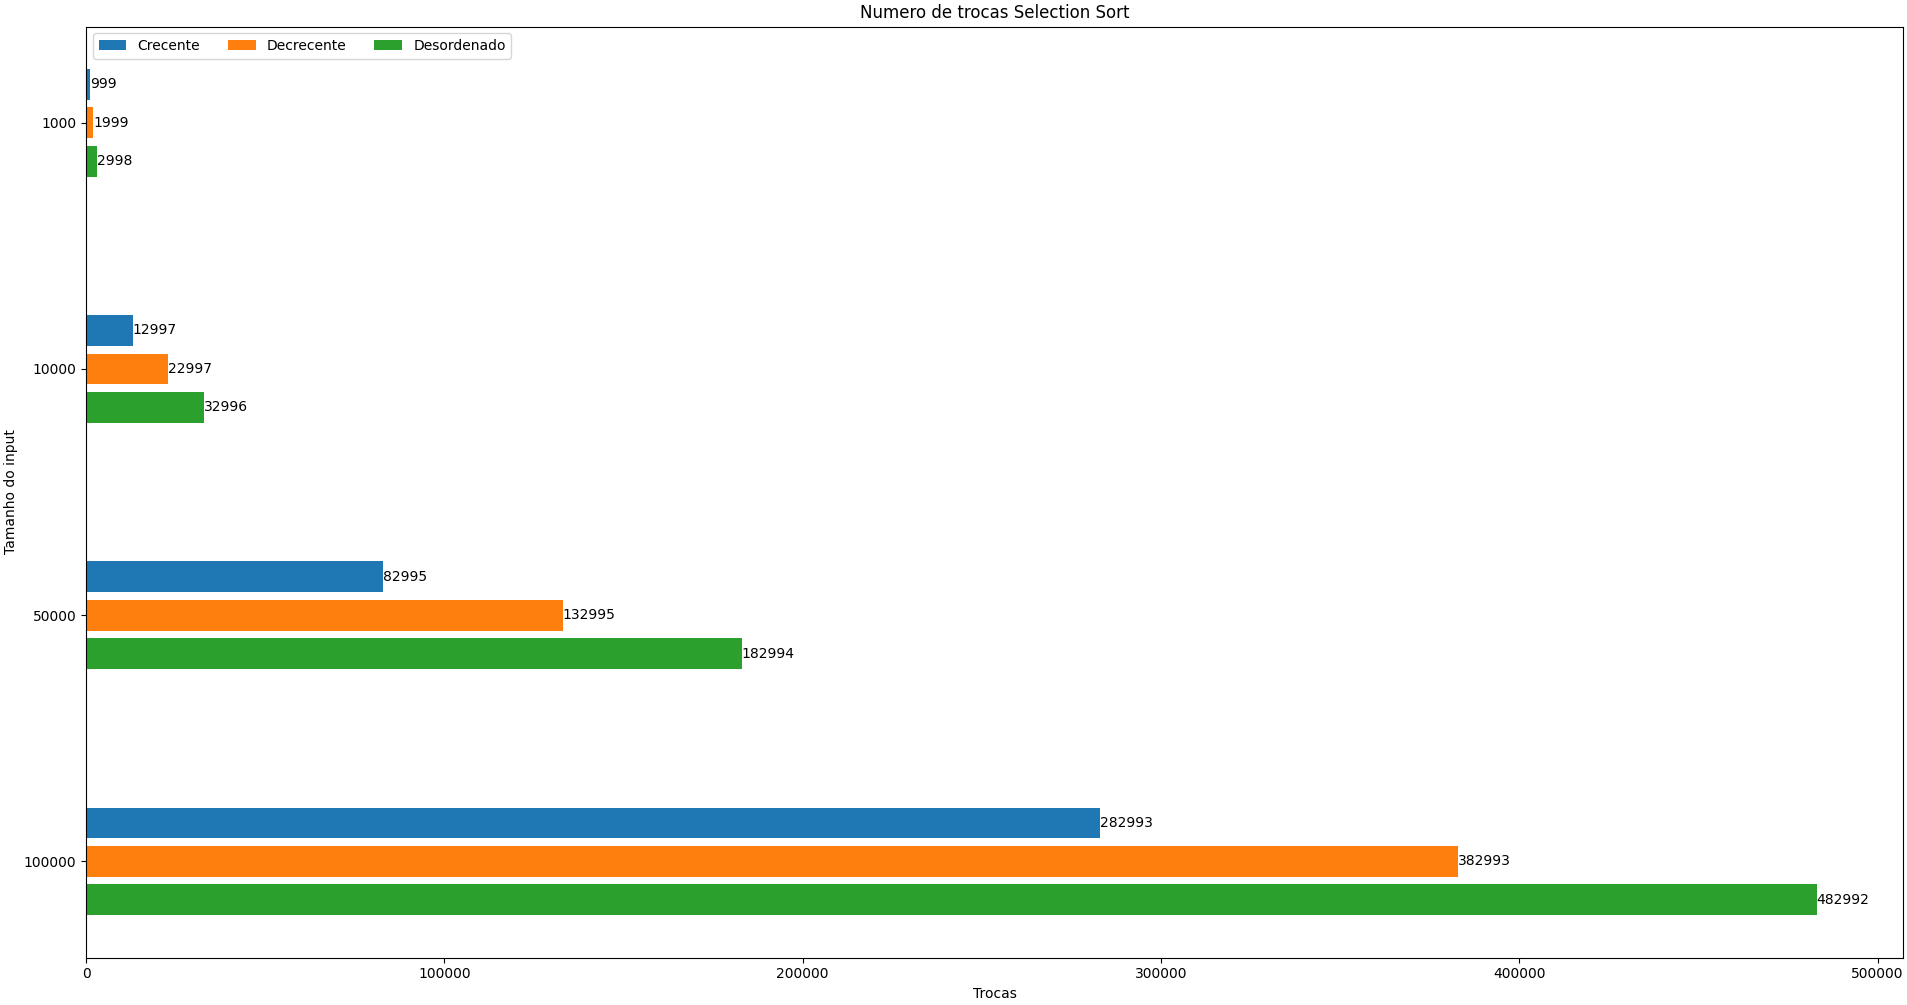
\includegraphics[width=\textwidth]{Graficos/Trocas/Selection Sort.png}
    \caption{Trocas Selection Sort}
    \label{fig:trocasSelectionSort}
\end{figure}


\section{Discussão}
\subsection{Análise dos Resultados}

\subsection{Heap Sort}
O Heap Sort apresenta um desempenho consistente, com tempos de execução que aumentam gradualmente com o tamanho dos dados. A diferença de tempo entre as entradas crescentes, decrescentes e desordenadas é mínima, o que é esperado, pois o Heap Sort tem um desempenho médio e pior de \(O(n \log n)\), independentemente da ordem de entrada.

\subsection{Insertion Sort}
O Insertion Sort apresenta tempos de execução muito baixos para entradas crescentes, que são esperados, pois o algoritmo funciona bem em listas já ordenadas. No entanto, para entradas decrescentes e desordenadas, os tempos de execução aumentam drasticamente, especialmente para tamanhos maiores, refletindo sua complexidade \(O(n^2)\) no pior caso.

\subsection{Merge Sort}
O Merge Sort apresenta um desempenho estável e consistente. Os tempos de execução para diferentes ordens são bastante próximos, o que confirma a expectativa teórica de que o Merge Sort opera em \(O(n \log n)\) em todos os casos. Isso o torna uma escolha sólida para listas de tamanhos maiores.

\subsection{Selection Sort}
Os resultados do Selection Sort confirmam a expectativa teórica de que ele é ineficiente, com tempos de execução elevados que aumentam rapidamente com o tamanho dos dados. Sua complexidade é \(O(n^2)\), o que se reflete nos altos tempos de execução observados, especialmente para entradas decrescentes e desordenadas.

\subsection{Bubble Sort}
O Bubble Sort, assim como o Selection Sort, demonstra um desempenho insatisfatório para entradas maiores. A complexidade \(O(n^2)\) é evidente em seus tempos de execução, especialmente para listas em ordem decrescente, onde o tempo se eleva a níveis preocupantes.

\subsection{Quick Sort Iterativo}
O Quick Sort Iterativo mostra um desempenho bastante eficiente para listas desordenadas, com tempos baixos comparados aos outros algoritmos. No entanto, para entradas crescentes e decrescentes, os tempos aumentam significativamente, especialmente em listas maiores. A complexidade média do Quick Sort é \(O(n \log n)\), mas sua complexidade no pior caso pode ser \(O(n^2)\), o que é visível nas diferenças de desempenho.


\subsection{Comparação com Expectativas Teóricas}
Os resultados obtidos confirmam amplamente as expectativas teóricas em relação aos algoritmos de ordenação. Algoritmos com complexidade \(O(n^2)\), como Bubble Sort, Insertion Sort e Selection Sort, apresentaram desempenhos inferiores, especialmente em entradas maiores e desordenadas. Em contraste, os algoritmos com complexidade \(O(n \log n)\), como Merge Sort, Quick Sort e Heap Sort, mantiveram um desempenho estável e eficiente, confirmando as previsões teóricas.

Uma observação interessante foi o desempenho do Quick Sort Iterativo. Embora seja eficiente na maioria dos casos, ele demonstrou vulnerabilidade em entradas ordenadas de forma crescente ou decrescente, confirmando a possibilidade de atingir a complexidade \(O(n^2)\) no pior caso. No entanto, as melhorias oferecidas por sua implementação iterativa se mostraram vantajosas em relação ao uso de memória.

\subsection{Considerações sobre Implementação e Uso de Memória}
Durante a implementação dos algoritmos, verificamos que o Merge Sort, apesar de eficiente em termos de tempo, exige um uso de memória adicional devido à necessidade de criar arrays temporários durante o processo de divisão e fusão dos dados. O Quick Sort Iterativo, por sua vez, mostrou-se mais eficiente em termos de uso de memória, eliminando a necessidade de recursão profunda.

Algoritmos como Heap Sort, que operam de forma in-place, demonstraram um uso mais otimizado da memória, o que o torna uma opção interessante quando o consumo de memória é uma limitação, embora seu tempo de execução seja um pouco maior em comparação ao Quick Sort em cenários ideais.

\subsection{Limitações do Trabalho}
Uma limitação importante deste trabalho foi o foco exclusivo no tempo de execução e no uso de memória. Aspectos como a facilidade de implementação e a adaptabilidade dos algoritmos a diferentes estruturas de dados não foram explorados. Além disso, não realizamos testes em conjuntos de dados muito grandes ou altamente específicos (como dados quase ordenados ou com padrões repetidos), o que poderia trazer insights adicionais sobre o comportamento dos algoritmos.

Outra limitação foi o ambiente de teste utilizado. Diferentes arquiteturas de hardware e configurações de sistema podem influenciar os tempos de execução, especialmente em algoritmos mais complexos como o Quick Sort e o Merge Sort.

\subsection{Sugestões para Estudos Futuros}
Para estudos futuros, sugerimos a análise de algoritmos de ordenação híbridos, como o TimSort, que combina o Merge Sort com o Insertion Sort para otimizar o desempenho em entradas parcialmente ordenadas. Também seria interessante explorar a eficiência dos algoritmos de ordenação em conjuntos de dados ainda maiores e em diferentes plataformas de hardware.

Outro aspecto a ser investigado é o impacto de paralelização dos algoritmos em ambientes de múltiplos núcleos ou distribuídos, especialmente para algoritmos como Quick Sort e Merge Sort, que podem se beneficiar significativamente de abordagens paralelas.

\section{Conclusão}
A análise dos resultados dos algoritmos de ordenação revela diferenças significativas em desempenho, dependendo da ordem e do tamanho dos dados. Algoritmos como Merge Sort e Quick Sort demonstram melhor desempenho em cenários gerais, enquanto Insertion Sort, Selection Sort e Bubble Sort são menos eficientes para listas maiores e desordenadas. A escolha do algoritmo adequado deve considerar as características da entrada e os requisitos de desempenho.

\subsection{Recomendações}
Com base nos resultados observados, recomendamos o uso do Merge Sort ou do Quick Sort para a maioria das aplicações práticas, especialmente quando o desempenho consistente em todos os cenários é crucial. O Heap Sort pode ser uma boa alternativa quando o uso de memória é uma preocupação. Por outro lado, algoritmos como Insertion Sort e Selection Sort são recomendados apenas para conjuntos de dados pequenos ou já quase ordenados, onde sua simplicidade e eficiência podem ser mais adequadas.

\section{Referências}
\begin{enumerate}
    \item Cormen, Thomas H., et al. *Introduction to algorithms*. MIT press, 2009.
    \item Sedgewick, Robert, and Kevin Wayne. *Algorithms*. Addison-Wesley Professional, 2011.
    \item Knuth, Donald E. *The art of computer programming: sorting and searching*. Vol. 3. Addison-Wesley Professional, 1998.
    \item Skiena, Steven S. *The algorithm design manual*. Springer Nature, 2020.
    \item Goodrich, Michael T., and Roberto Tamassia. *Algorithm design and applications*. John Wiley \& Sons, 2014.
    \item McIlroy, M. Douglas. "A killer adversary for quicksort." *Software-Practice and Experience*, vol. 29, no. 4, 1999, pp. 341-344.
\end{enumerate}

\end{document}